\section{Eksperimenti 2. faze}
Z laboratorijskimi eksperimenti v 1. fazi smo dobili zadovoljive rezultate, težave pa so nastale pri uporabi postopka na terenu. Zato smo v 2. fazi optimizirali posamezne segmente elementarnega postopka estimacije fizioloških parametrov. Te smo tudi uporabili v končni preiskavi. V preliminarnih testih so opisani tudi drugi postopki, ki smo jih potrebovali zaradi uporabe Kinect kamer.

Za statistično bolj oprijemljive rezultate smo v laboratorijskih in terenskih eksperimentih 2. faze uporabili 7 različnih merjencev  ($srednja vrednost \pm SD$: starost $16.29 \pm 2.29$ let, velikost $175.37 \pm 11.60$ \si{\cm}, teža $59.36 \pm 12.08$ \si{\kg}, spol moški, $hr_{max}$ $203.71 \pm 2.29$ \si{bpm}, \vomax $3144 \pm 629.27$ \si{\ml\per\min} ) z oznakami: SUBJ1, SUBJ2, SUBJ4, SUBJ7, SUBJ8, SUBJ9, SUBJ10. 

Merjenca SUBJ4 smo uporabili samo v laboratorijskih eksperimentih, ker pri terenskih eksperimentih ni bil prisoten. Namesto njega smo v terenskih eksperimentih uporabili merjenca SUBJ10. V laboratorijskih eksperimentih merjenca SUBJ10 nismo upoštevali zaradi napak pri zajemu meritev.

Med laboratorijskimi in terenskimi eksperimenti je za merjenca SUBJ1 in SUBJ2 preteklo 43 dni, za merjenca SUBJ4 42 dni in za ostale 1 dan.  

\subsection{Mrežno iskanje \texorpdfstring{$\nu$}{nu}-RBF}
Med evaluacijo eksperimentov 1. faze smo ugotovili, da z regresijo \esvr pogosto dobimo preobremenjene (ang. Overfitted) modele. Pri takih modeli je število podpornih vektorjev zelo visoko. Lahko se zgodi, da postanejo vsi vektorji značilk podporni vektorji. Preobremenjeni modeli lahko dajejo solidne rezultate, vendar pa so ti nerealistični. Takoj, ko bi v tak model vnesli rahlo spremenjene podatke, ne bi več delovali.

Zaradi tovrstnih problemov smo v našem postopku regresijo \esvr zamenjali z \nusvr. Izkazalo se je, da tudi ta ne deluje, čeprav pri njej uporabljamo dodatni parameter $\nu$, s katerim v teoriji kontroliramo razmerje števila podpornih vektorjev, kot je opisano v poglavju~\ref{sec:regresija-nusvr}. Chang et. al nam v delu~\cite{chang2002training} parameter $\nu$ bolj natančno opiše kot spodnjo mejo razmerja števila podpornih vektorjev. Parameter $\nu$ tako v resnici ne predstavlja omejitve, s katero bi kaznovali prekomerno učenje modela. V ta namen smo razvili mrežno iskanje \nurbf, ki je predstavljeno v poglavju~\ref{sec:nurbf}. 

Razvito mrežno iskanje uporablja regresijo \nusvr in jedro RBF, zato smo ju uporabljali tudi za učenje modelov. Celoten postopek krajše imenujemo kar \nurbf.


\paragraph{Optimizacija parametrov}
Najprej smo optimizirali parameter $\numax$. Slednji predstavlja različico parametra $\numax$, s katerim določimo dejansko število podpornih vektorjev. Za tovrstno optimizacijo smo ponovno naučili \textit{mixed} modele iz 1. faze, pri čemer smo za mrežno iskanje uporabili nov postopek. Modele smo nato uporabili za testiranje na učnih podatkih terenskih eksperimentov 1. faze. S takim postopkom smo izluščili slabe \textit{squash} modele, ki bi oteževali pravilno evaluacijo rezultatov pri optimizaciji.

Za optimizacijo smo uporabili HOOF-HAFA deskriptor in naslednje vrednosti parametrov: začetna vrednost $\nu$ $0.1$, skaliranje značilk na intervalu $[-1,~1]$ in standardni odklon za Gaussov filter $\sigma=5$. Za $\numax$ smo uporabili \num{0.2}, \num{0.5} in \num{0.8}. Pri evaluaciji smo uporabili rezultate verifikacije in ne validacije, kot običajno. Pri validaciji smo dobili slabe rezultate iz katerih nismo mogli sklepati o izbiri optimalnega parametra.

\paragraph{Primerjava z elementarnim postopkom 1. faze}
Z optimiziranim parametrom $\numax=0.5$, smo \nurbf preizkusili še na elementarnih modelih, pri čemer nismo upoštevali izrezovanja slik. Ostali parametri so enaki kot pri optimizaciji



\subsection{Optimizacija Gaussovega filtra}
Pri optimizaciji Gaussovega filtra smo določili optimalni standardni odklon $\sigma$ z uporabo dveh metrik, in sicer: koren srednje kvadratične napake (RMSE) in razmerje med signalom in šumom (SNR). Pri RMSE metriki smo določili napako med učnimi vzorci in njihovo predikcijo. Pri SNR metriki smo za signal uporabili referenčne učne vzorce. Za šum smo uporabili rezidualni ali preostali šum. Tega smo dobili z odštevanjem filtriranih vzorcev od referenčnih. SNR metrika tako določa uspešnost izločevanja šuma, RMSE metrika pa pravilnost določevanja kateri podatki spadajo v signal in kateri v šum.

Teste smo izvajali na elementarnih eksperimentih 1. faze brez upoštevanja izrezovanja slik, pre čemer smo uporabili HOOF-HAFA deskriptor. Značilke smo skalirali na intervalu $[0,~1]$, ker smo pri uporabi intervala $[-1,~1]$ dobili opozorila, naj raje uporabimo prvega. Za postopek učenja smo izbrali \nurbf z \hbox{$\numax=0.5$} in \hbox{$\sigma=1$}. Testirali smo naslednje standardne odklone Gaussovega filtra: $1, 3, 5, 11, 21, 31$ in $51$. 


\begin{comment}
\subsubsection{Jedro GHI}
V poglavju~\ref{sec:ghi} smo opisali, da je jedro GHI primerno za histogramske deskriptorje, zato smo ga tudi preizkusili na elementarnih modelih brez upoštevanja izrezovanja slik. Namesto prvotnega HOOF deskriptorja smo uporabili HOOF-HAFA deskriptor, ki daje boljše rezultate. Pri uporabi GHI jedra smo značilke skalirali na intervalu $[-1,~1]$ zaradi hitrejšega učenja. Uporabili smo postopek \nughi. Gre za prilagojeno različico postopka \nurbf, kjer smo uporabili GHI jedro. %Dodatna razlika je še v tem, da predikcij pri križni validaciji nismo filtrirali. S tem zagotovili zadovoljiv čas reševanja problema. 
Pri postopku smo uporabili $\numax=0.5$ in $\sigma=5$. Rezultate smo filtrirali s prvotnim Gaussovim filtrom $\sigma=5$.

%Zaradi že prej omenjenih težav s prevelikim številom podpornih vektorjev v modelih, smo pri klasičnem mrežnem iskanju sprva uporabili enostavno mero: faktor števila podpornih vektorjev $f_{nSV}$, ki je opisan z enačbo~\eqref{eq:fnsv}. $n_v$ je število vzorcev in $n_{SV}$ je število podpornih vektorjev. S to mero določimo procentualno vrednost vektorjev, ki lahko postanejo podporni. Zaradi tega faktorja optimizacija parametra regresije ni bila potrebna. Pri testiranju smo uporabili vrednost $f_{nSV} = 0.01$.


%\begin{equation}
%f_{nSV} = \frac{n_v - n_{SV}}{n_v}
%\label{eq:fnsv}
%\end{equation} 
\end{comment}


\subsection{Normalizacija HAFA deskriptorjev}
V praksi se pokaže, da prvotni HAFA histogram ne deluje zadovoljivo, saj se histogram lahko močno spreminja pri uporabi sledilnika. Zaradi neidelanega delovanja sledilnika področje tarče skozi čas spreminja svojo velikost, to pa vpliva na vrednosti stolpcev HAFA histograma. Ker te dobimo s preštevanjem slikovnih elementov z enako amplitudo hitrosti bo manjše področje posledično zmanjšalo celoten histogram. Pri HOOF histogramih tega problema praktično nimamo, saj ima majhen vpliv. Razlog tiči v računanju vrednosti stolpcev HOOF histograma. Njihove vrednosti dobimo s seštevanjem amplitud in ne njihovim preštevanjem. Te so zato pred normiranjem praviloma večje.

Probleme sledilnika smo poskušali kompenzirati z uvedbo amplitudnega faktorja $f_A$. Amplitudni faktor je pravzaprav razmerje med velikostjo področja igralca na terenskih testih in velikostjo merjenca na tekalni stezi. Razmerje lahko preprosto dobimo z razmerjem diagonal področij po enačbi~\eqref{eq:diag}, kjer so $w_l$ in $h_l$ širina in dolžina področja na tekalni stezi ter $w_s$ in $h_s$ širina in dolžina področja na terenskih testih.

\begin{equation}
f_A = \frac{\sqrt{w_l^2 + h_l^2}}{\sqrt{w_s^2 + h_s^2}}
\label{eq:diag}
\end{equation}

Velikost diagonale na laboratorijskih testih uporabljamo kot referenco. To pa zato, ker je na teh posnetkih stabilna, saj se le malo spreminja. Koncept amplitudnega faktorja smo preizkusili na enakem postopku, kot pri optimizaciji parametra mrežnega iskanja \nurbf. S takim postopkom smo izluščili slabe \textit{squash} modele, ki bi oteževali pravilno evaluacijo rezultatov pri optimizaciji. Naučili smo modele \textit{diag}, kjer smo uporabili amplitudni faktor in referenčne modele \textit{normal} brez uporabe faktorja za primerjavo. Diagonalo na tekalni stezi smo določili po sliki~\ref{fig:diag-bbox}, kjer smo za zgornji levi kot $P_0$ in spodnji desni kot $P_1$ izbrali vrednosti v tabeli~\ref{tab:diag}. 


\begin{figure}[!htb]
	\centering
	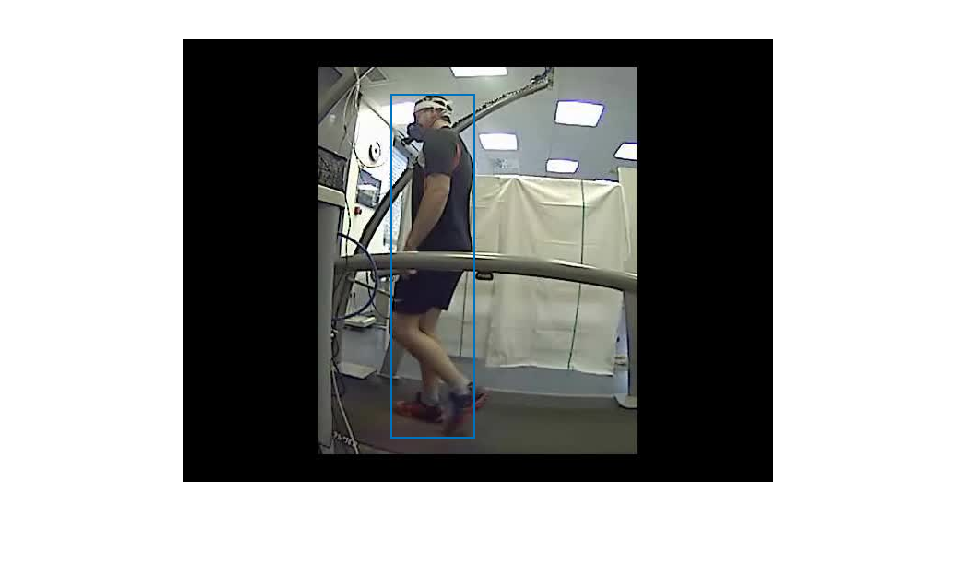
\includegraphics[width=0.75\columnwidth]{diag-bbox.png}
	\caption[Določitev amplitudnega faktorja]{Določitev amplitudnega faktorja. Amplitudni faktor $f_A$ smo določili kot dolžino diagonale modrega okvirja. Modri okvir smo določili ročno.}
	\label{fig:diag-bbox}
\end{figure}

\begin{table}[!htb]
	\centering
	\begin{tabular}{l S[table-format=3] S[table-format=3]}
		\toprule
		\textbf{Točka} & \theadm{x} & \theadm{y} \\ 
		\midrule
		$P_0$ & 297 & 82 \\
		$P_1$ & 389 & 452 \\
		\bottomrule
	\end{tabular}
	\caption[Tabela izbranih točk okvirja za amplitudni faktor]{Tabela izbranih točk okvirja merjenca, s katerimi smo določili amplitudni faktor. Točka $P_0$ je zgornji levi kot točka $P_1$ pa spodnji levi kot modrega okvirja na sliki~\ref{fig:diag-bbox}}
	\label{tab:diag}
\end{table}

Pri testiranju smo uporabili parameter $\numax = 0.5$ in $\sigma=5$. Za filtriranje meritev srčnega utripa smo uporabili $\sigma=16$ za rezultate pa optimalno vrednost $\sigma=5$. Značilke smo skalirali na intervalu $[0,~1]$,  ker smo pri uporabi intervala $[-1,~1]$ dobili opozorila, naj raje uporabimo prvega. Za modele z diagonalo smo uporabili parameter $f_{A}=381.266$. Pri učenju smo uporabili optimalne vrednosti parametrov, ki so prikazane v tabeli~\ref{tab:diag}. Za evaluacijo rezultatov smo uporabili predikcije testnih vzorcev z modeli s zakasnitvijo.



\begin{table}[htb]
	\centering
	\begin{tabular}{l S[table-format=3] S[table-format=1.3] S[table-format=1.1] S[table-format=1.3]}
		\toprule
		\textbf{Model} & \theadm{C} & \theadm{\gamma} & \theadm{\nu} & \thead{MSE} \\
		\midrule
		NORMAL & 256 & 0.354 & 0.1 & 5.297 \\
		DIAG & 256 & 0.354 & 0.1 & 5.297 \\
		\bottomrule
	\end{tabular}
	\caption[]{Optimalni parametri pri učenju modela brez upoštevanja amplitudnega faktorja NORMAL in modelu s faktorjem DIAG.}
	\label{tab:izbira-param-diag}
\end{table}


\subsection{Laboratorijski eksperimenti}
Merjenci so opravili obremenilni test po protokolu Nowatzky. To je stopnjevani test na tekoči preprogi za merjenje maksimalne porabe kisika in oceno aerobne kapacitete posameznika.

\subsubsection{Pridobivanje podatkov}
\paragraph{Fiziolo\v{s}ki parametri.}
Obremenilni test smo izvajali s pomočjo sistema za direktno ergospirometrijo tipa ``breath  by breath'' Cosmed K4B2. Uporabili smo  tekočo  preprogo HP Cosmos. Z obremenilnim testom smo pridobili podatke energijske porabe šestih različnih merjencev z oznakami: SUBJ1, SUBJ2, SUBJ4, SUBJ7 SUBJ8 in SUBJ9. Vzorčili smo s frekvenco \SI{0.2}{\hertz}.

\paragraph{Video posnetki.}
Tekalno stezo smo snemali iz dveh različnih zornih kotov: hrbtni del in stranski del. Kameri sta bili časovno sinhronizirani po NTP protokolu. Frekvenci vzorčenja na posamezni kameri sta se rahlo spreminjali, zato smo pridobivali tudi časovne štampiljke slik posnetkov. Z njimi smo posnetka dodatno sinhronizirali in se znebili akumulacije časovnega zamika.  Primer hrbtnega in stranskega posnetka je prikazan na sliki~\ref{fig:primer-posnetka-stage2}.

\begin{figure}[!htb]
	\centering
	\begin{subfigure}{0.45\columnwidth}
		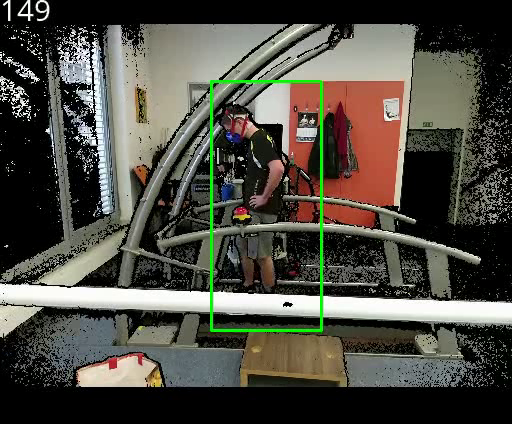
\includegraphics[width=\columnwidth]{stage2-lab-sv-tracked.png}
		\caption{Stranska slika.}
	\end{subfigure}
	~
	\begin{subfigure}{0.45\columnwidth}
		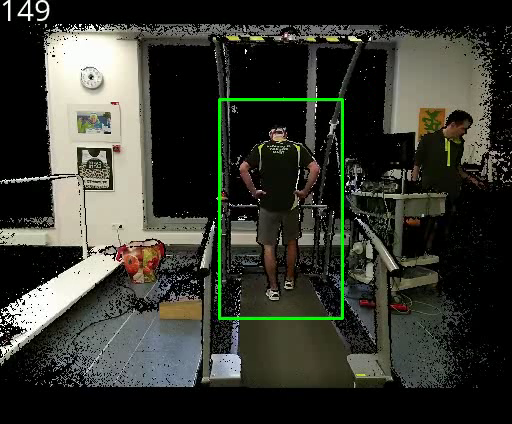
\includegraphics[width=\columnwidth]{stage2-lab-bv-tracked.png}
		\caption{Hrbtna slika.}
	\end{subfigure}
	\caption[Stranski in hrbtni posnetek iz Kinect kamere v laboratoriju]{Stranski in hrbtni posnetek iz Kinect kamere v laboratoriju. Sliki sta bili registrirani na korespondečni globinski sliki~\ref{fig:stage2-lab-of-depth}. Črni slikovni elementi predstavljajo točke, kjer globina ni bila pravilno zajeta. Zeleni okvir je rezultat sledenja s KCF sledilnikom.}
	\label{fig:primer-posnetka-stage2}
\end{figure}

Snemali smo z dvema Microsoft Xbox Kinect V2 kamerama. Kameri sta bili od tekalne steze oddaljeni približno \SI{2}{m}. Od tal sta bili dvignjeni za približno \SI{1.5}{m}. Postavitev kamer je prikazana na sliki~\ref{fig:lab-postavitev-kamer}. Pridobili smo barvne RGB in globinske DEPTH slike. Snemali smo v ločljivosti $512 \times 424$. Hitrost posnetkov je znašala \SI{30}{fps}.

\begin{figure}[!htb]
	\centering
	\begin{subfigure}[t]{0.45\columnwidth}
		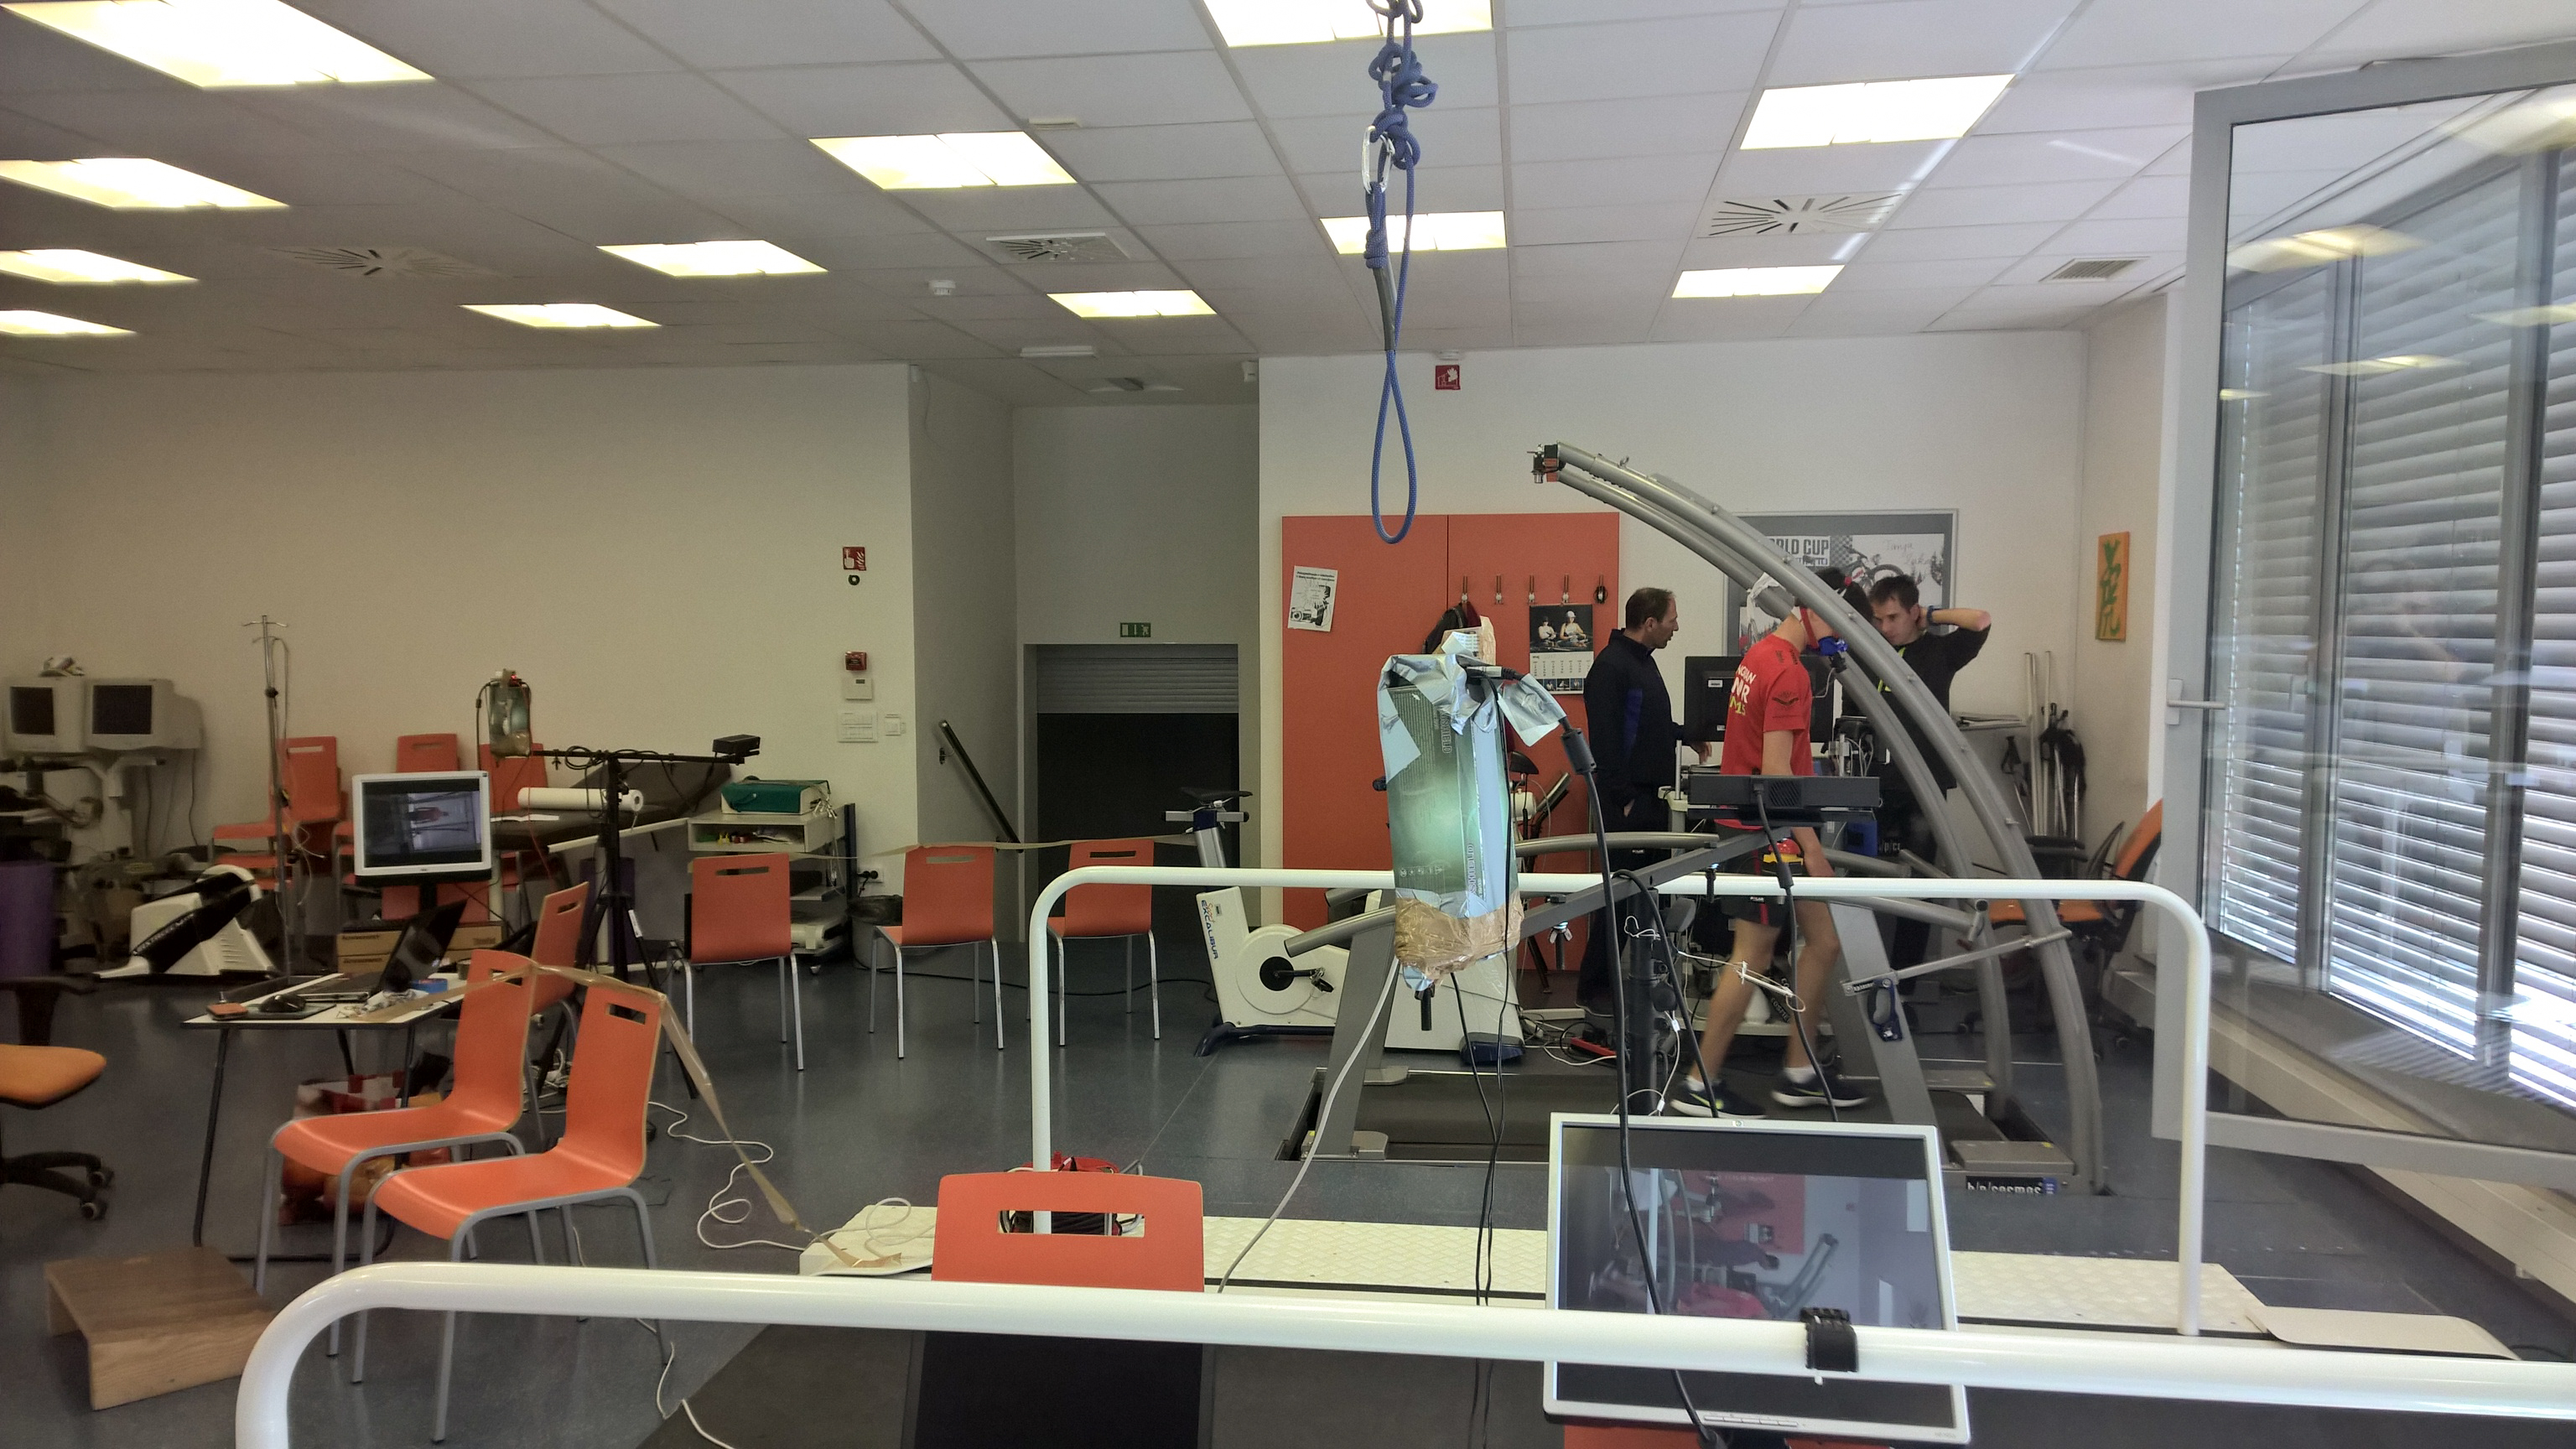
\includegraphics[width=\columnwidth]{lab-posnetek-iz-strani-corrected.jpg}
		\caption{Stranski pogled.}
	\end{subfigure}
	~
	\begin{subfigure}[t]{0.45\columnwidth}
		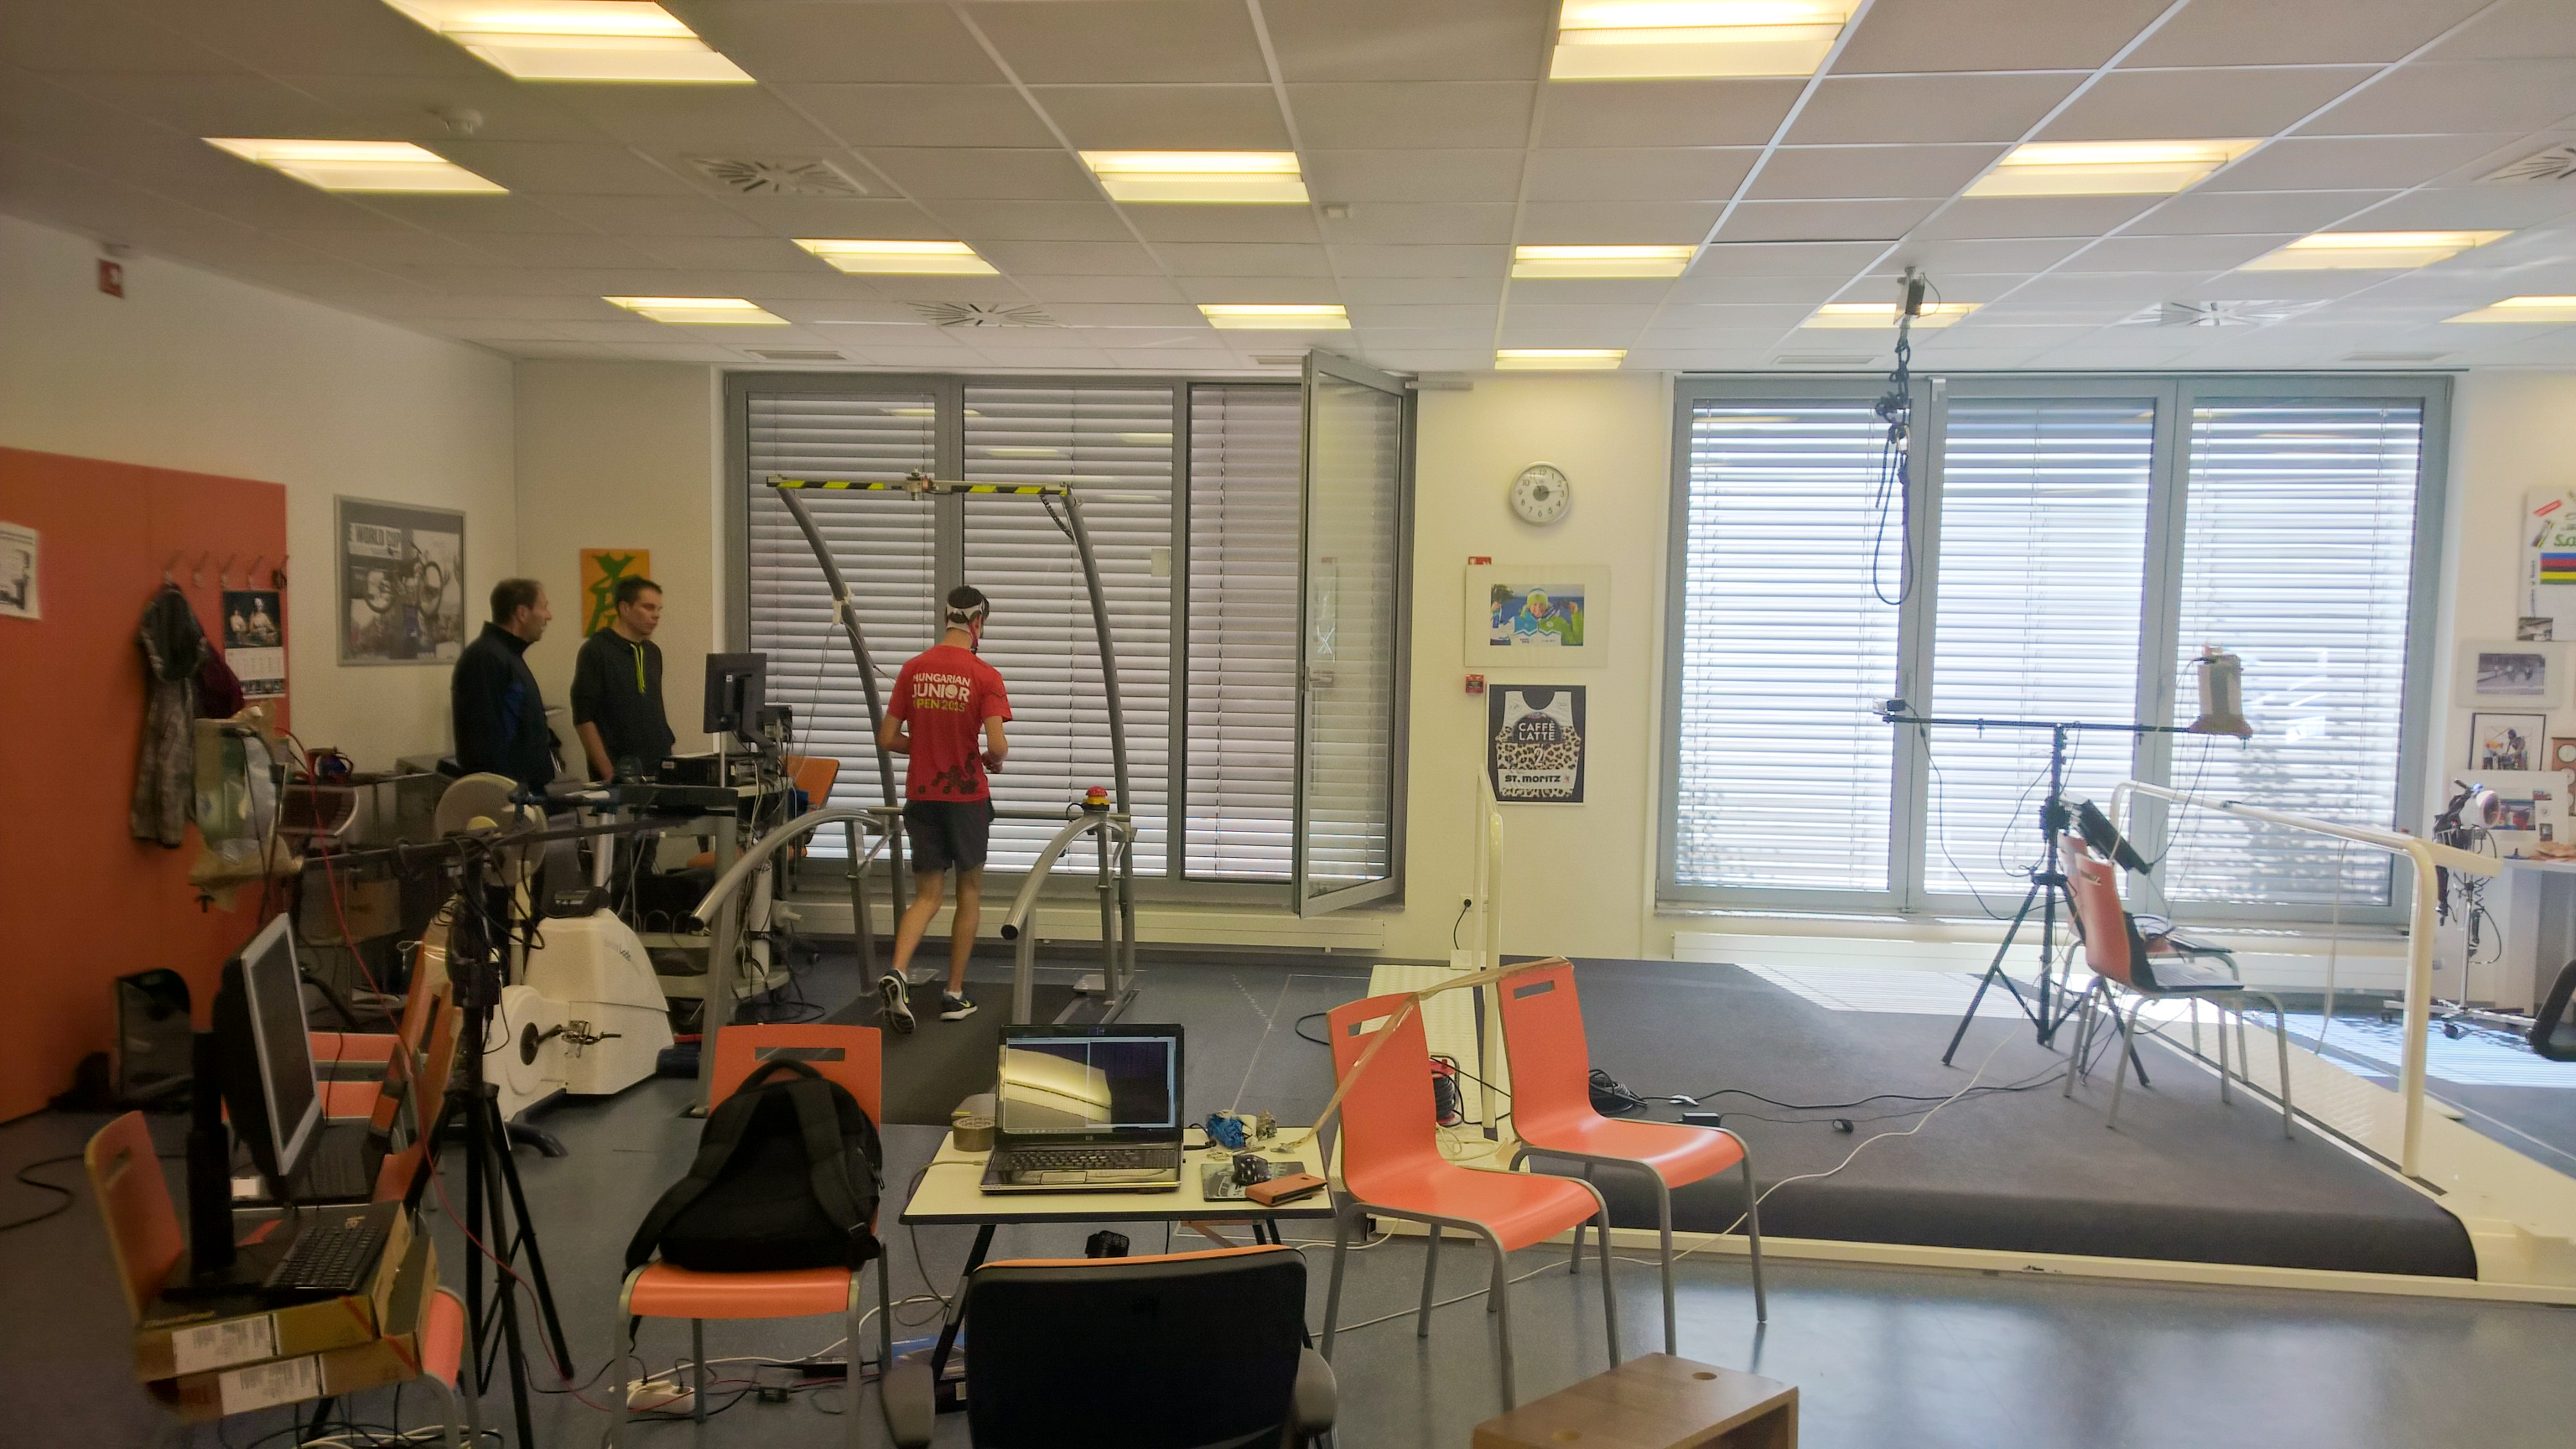
\includegraphics[width=\columnwidth]{lab-posnetek-zadaj-corrected.jpg}
		\caption{Hrbtni pogled.}
	\end{subfigure}
	\caption[Stranski in hrbtni pogled izvajanja lab. testov 2. faze]{Stranski in hrbtni pogled postavitve kamer za laboratorijske teste 2. faze. Na sliki sta vidna podstavka, na katerih so postavljene Kinect kamere. Kameri sta bili od tekalne steze oddaljeni približno \SI{2}{m}.}
	\label{fig:lab-postavitev-kamer}
\end{figure}


\begin{figure}[!htb]
	\centering
	\begin{subfigure}[t]{0.45\columnwidth}
		\centering
		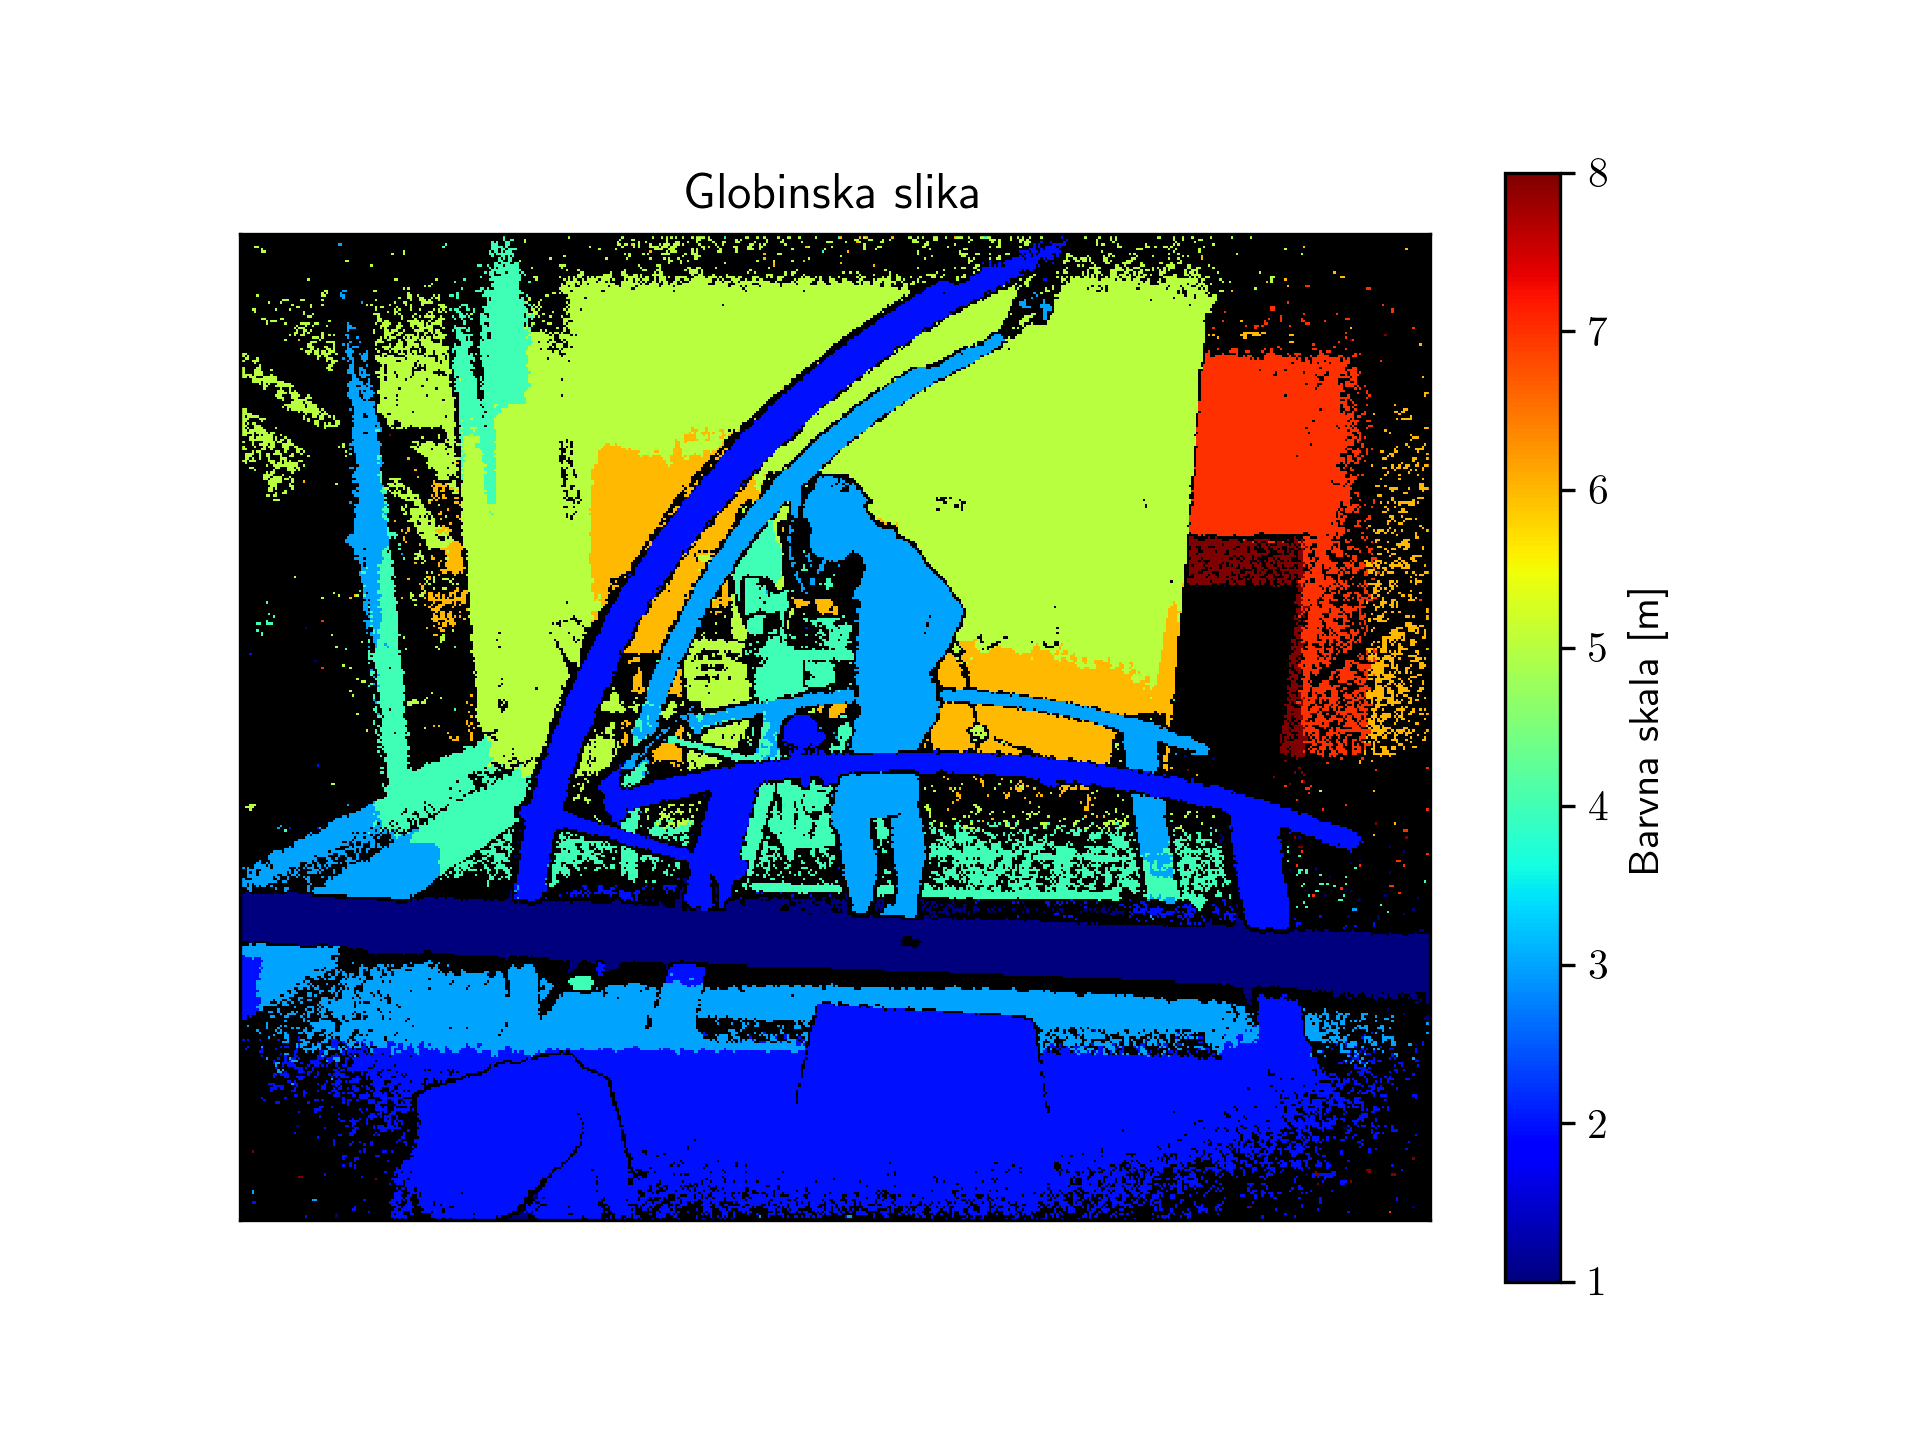
\includegraphics[width=1.2\columnwidth]{stage2-lab-sv-depth-sl}
		\caption{Stranska slika.}
	\end{subfigure}
	~
	\begin{subfigure}[t]{0.45\columnwidth}
		\centering
		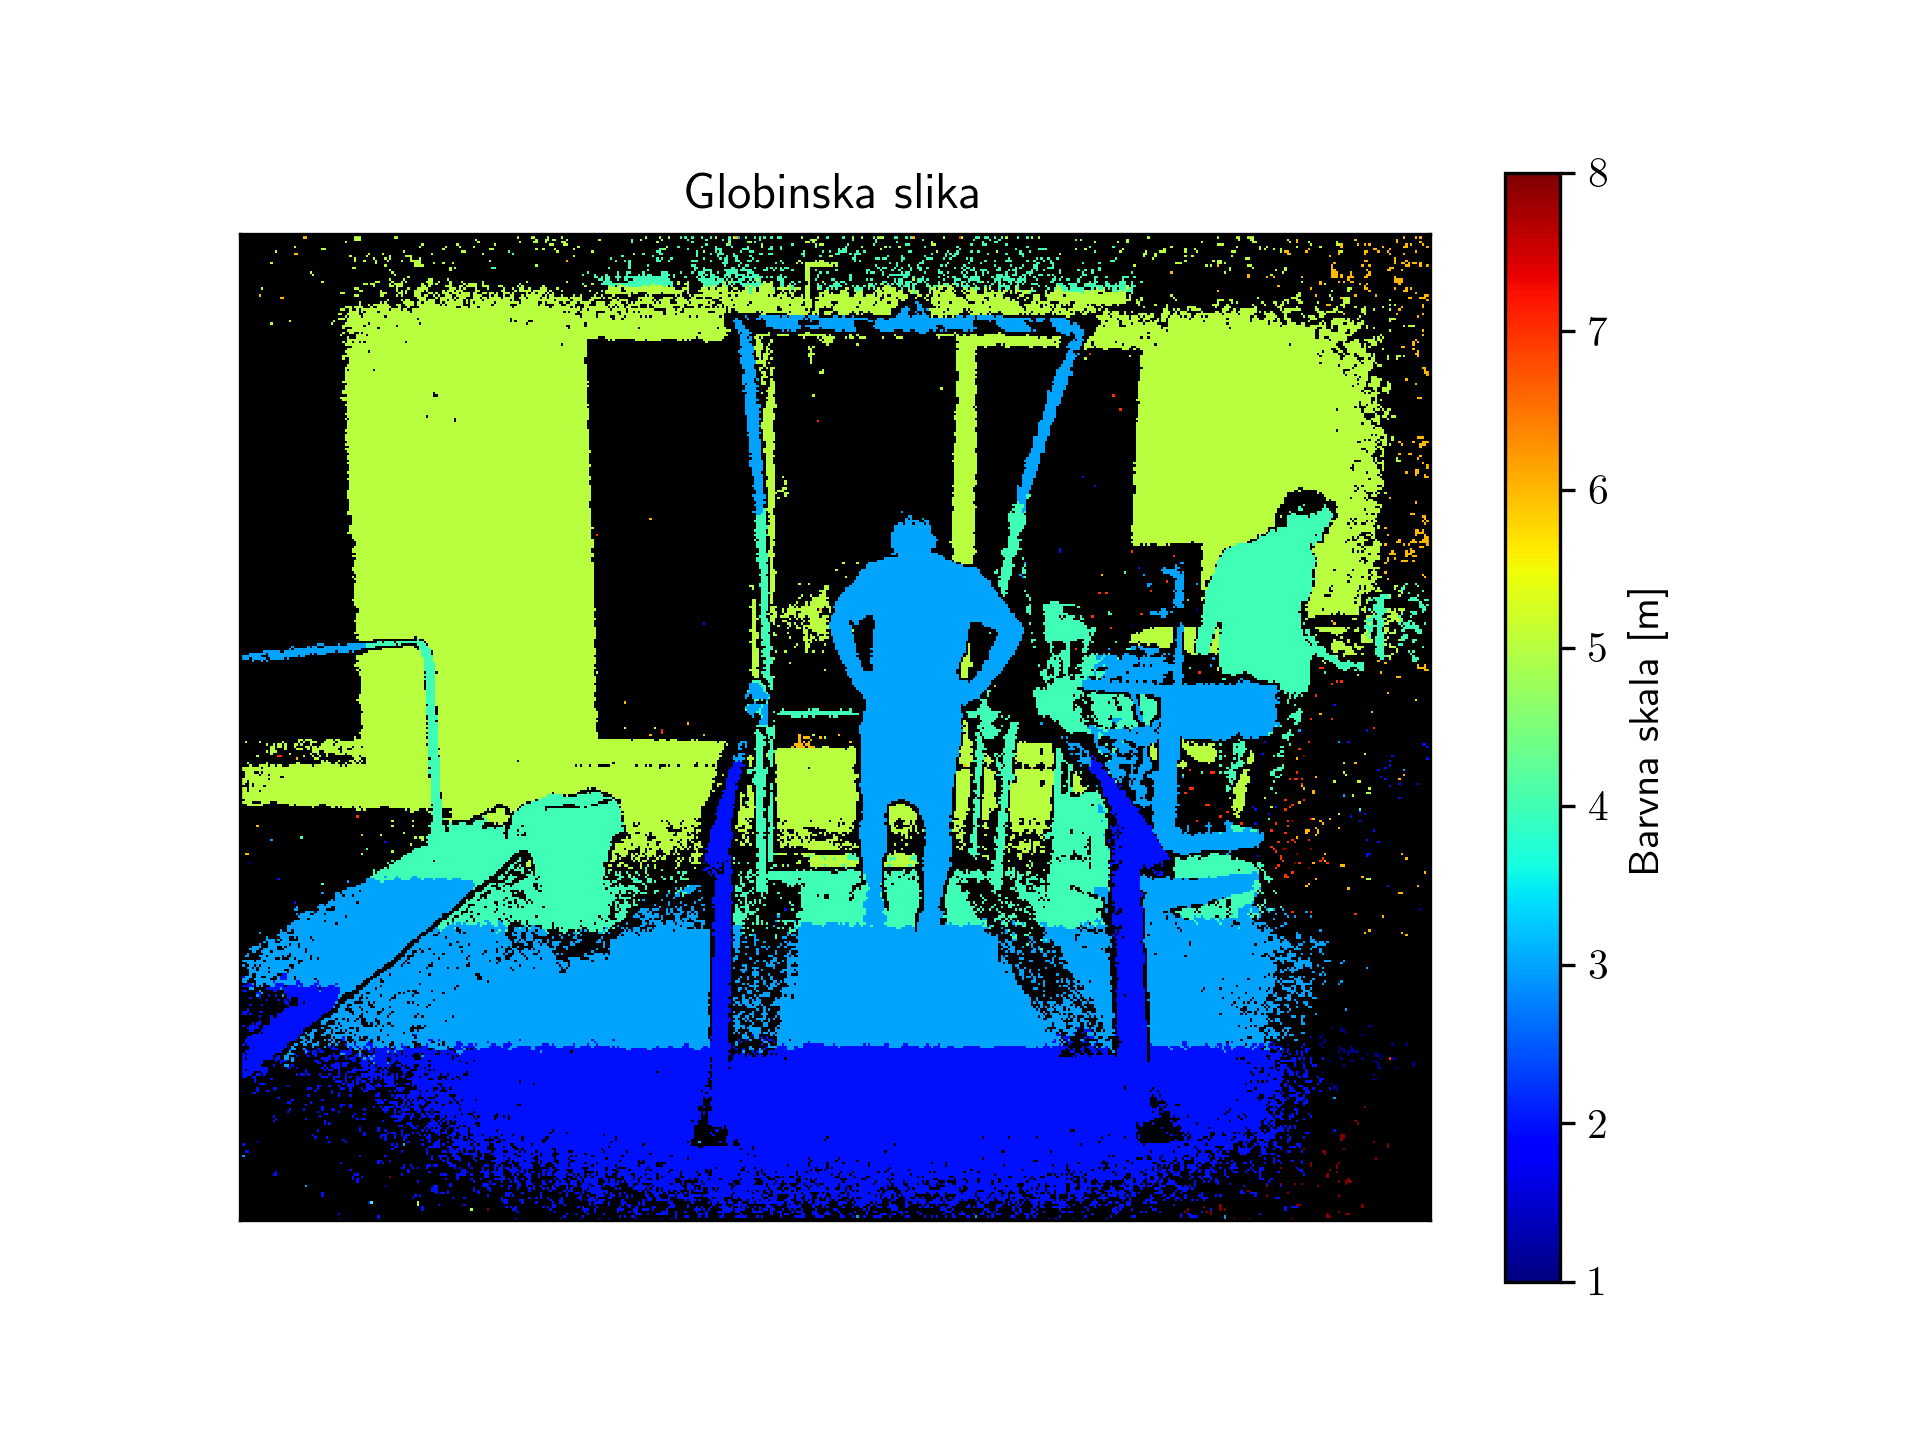
\includegraphics[width=1.2\columnwidth]{stage2-lab-bv-depth-sl}
		\caption{Hrbtna slika.}
	\end{subfigure}
	\caption[Stranska in hrbtna globinska slika laboratorijskih eksperimentov]{Stranska in hrbtna globinska slika laboratorijskih eksperimentov. Globinski sliki sta korespondečni RGB slikam~\ref{fig:primer-posnetka-stage2}. Barvna skala prikazuje globino v metrih. Črni slikovni elementi predstavljajo točke, kjer globina ni bila pravilno zajeta.}
	\label{fig:stage2-lab-of-depth}
\end{figure}



\paragraph{Protokol meritev.}
Test smo pričeli z eno minutnim mirovanjem na tekalni stezi. Sledilo je tri minutno ogrevanje s hitrostjo teka \SI{5}{\km\per\hour}, pri naklonu preproge \SI{0}{\%}. Nadaljevali smo s 3 minutnim tekom s hitrostjo \SI{6}{\km\per\hour}. Po treh minutah smo naklon tekoče preproge  dvignili za \SI{2}{\%} in ga nismo več spreminjali. Po pretečeni minuti na  tretji stopnji (hitrost \SI{6}{\km\per\hour}, naklon \SI{2}{\%}) se je hitrost teka vsaki dve  minuti  povečevala za \SI{1}{\km\per\hour}. Test smo izvajali brez prekinitve do pojava objektivnih oz. subjektivnih razlogov za prekinitev testa. 
%Po koncu testiranja je sledilo še \SI{5}{min} hoje pri  hitrosti \SI{2}{\km\per\hour} ter \SI{0}{\%} naklonu. 
 

\subsubsection{Procesiranje}
Zaradi razlik frekvenc vzorčenja, smo fiziološke parametre interpolirali s pomočjo Matlabove funkcije \texttt{interp1}. Modele smo učili po dveh postopkih. Prvi postopek temelji na optičnem toku, drugi pa na prostorskem.

\paragraph{Postopek z optičnim tokom}
Na slikah posnetkov smo merjencem sledili s sledilnikom KCF. Za tako izbrano področje slike smo izračunali optični tok. Primer dobljenega optičnega toka je prikazan na sliki~\ref{fig:opticni-tok-stage2}. Sledilo je generiranje HOOF-HAFA deskriptorjev s parametri $N_{HOOF} = 60$ in $N_{HAFA} = 60$. HAFA deskriptorje smo normalizirali z vrednostmi amplitudnih faktorjev $f_A$, ki so zbrani v tabeli~\ref{tab:fa-merjenci}.


\begin{figure}[!htb]
	\centering
	\begin{subfigure}[t]{0.45\columnwidth}
		\centering
		
\includegraphics[width=0.5\columnwidth, frame]{stage2-lab-of-sv-flo-corrected.png}
		\caption{Stranska slika.}
		\label{fig:stage2-lab-of-sv-flo}
	\end{subfigure}
	~
	\begin{subfigure}[t]{0.45\columnwidth}
		\centering
		
\includegraphics[width=0.5\columnwidth, frame]{stage2-lab-of-bv-flo-corrected.png}
		\caption{Hrbtna slika.}
		\label{fig:stage2-lab-of-bv-flo}
	\end{subfigure}
	~
	\begin{subfigure}[t]{0.45\columnwidth}
		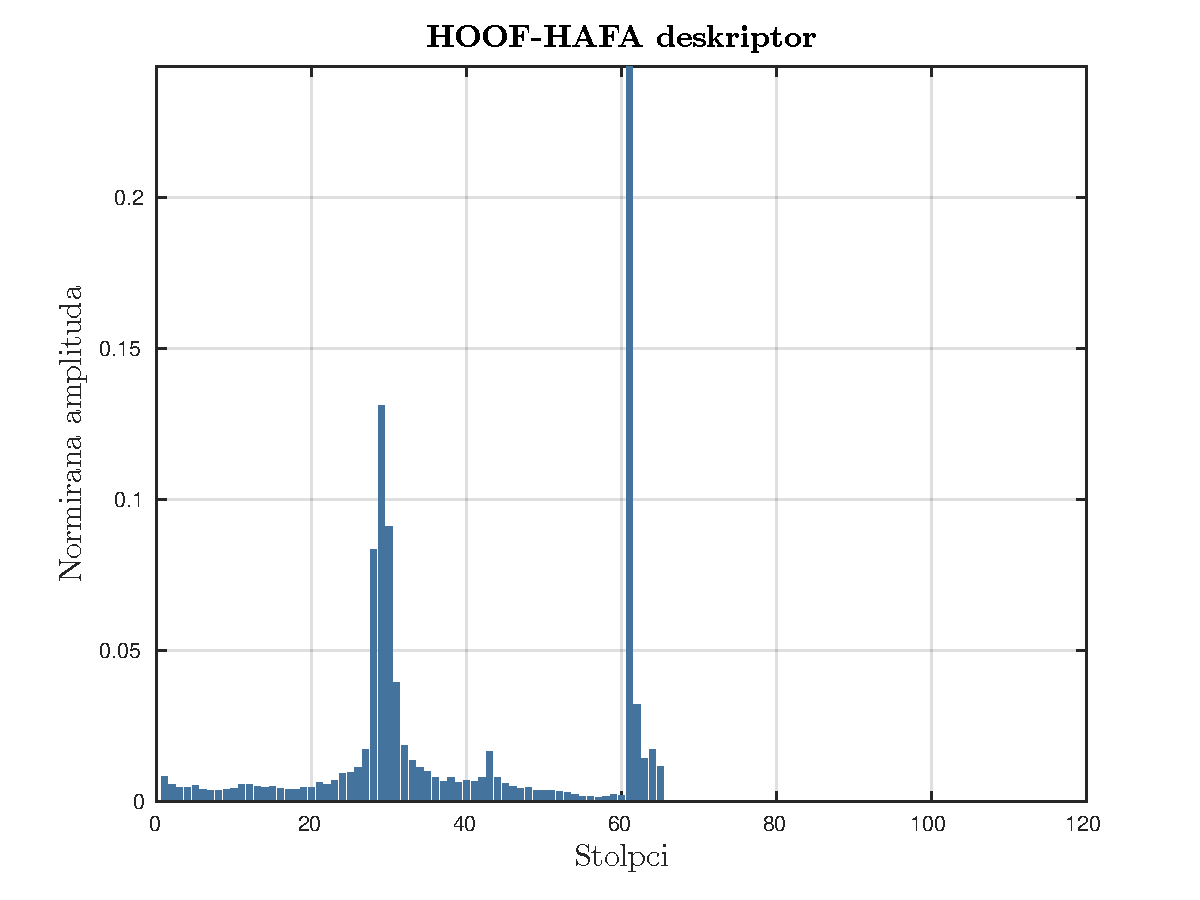
\includegraphics[width=\columnwidth]{stage2-lab-sv-of-hist-sl}
		\caption{Histogram stranske slike.}
	\end{subfigure}
	~
	\begin{subfigure}[t]{0.45\columnwidth}
		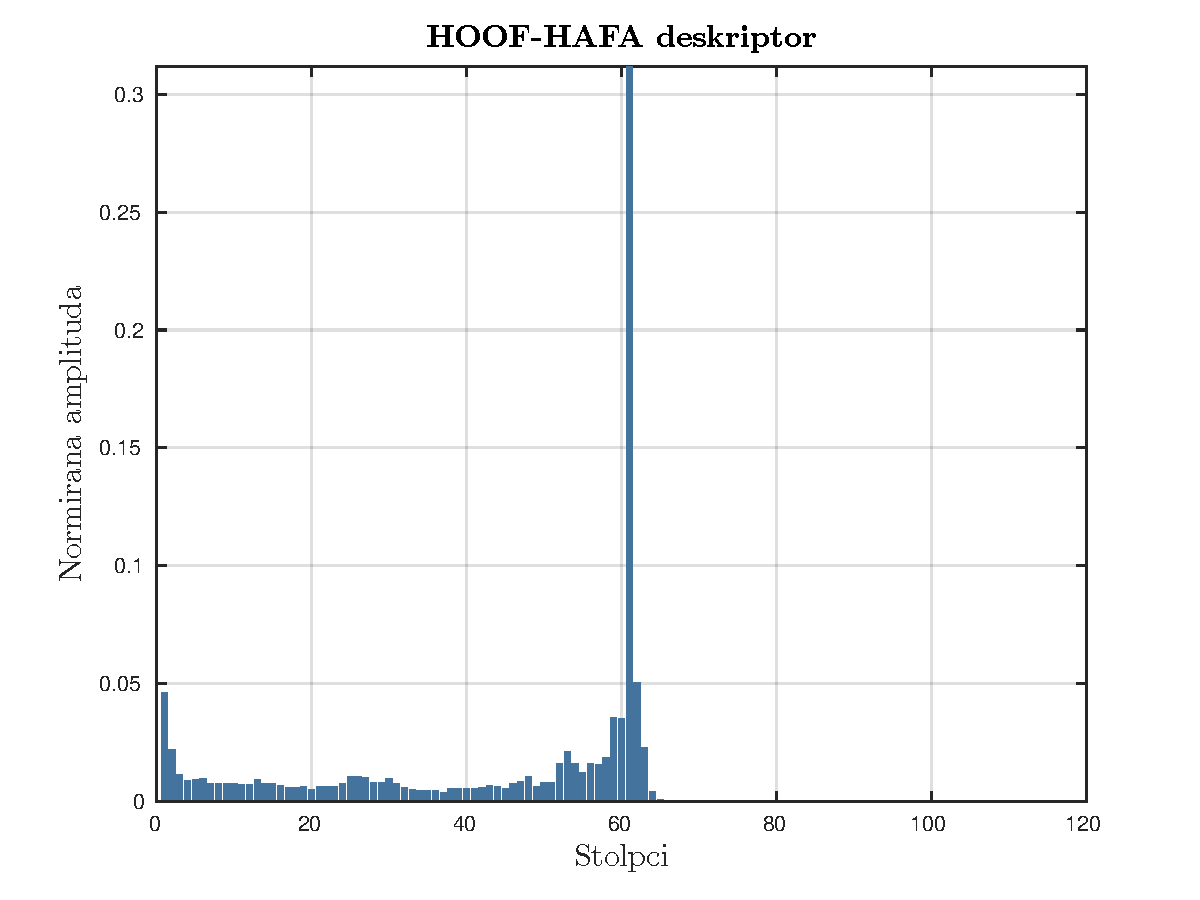
\includegraphics[width=\columnwidth]{stage2-lab-bv-of-hist-sl}
		\caption{Histogram hrbtne slike.}
	\end{subfigure}
git    \caption[Stranski in hrbtni optični tok ter pripadajoča deskriptorja]{Stranski in hrbtni optični tok ter pripadajoča deskriptorja. Sliki \subref{fig:stage2-lab-of-sv-flo}) in \subref{fig:stage2-lab-of-bv-flo}) sta optična toka 24. stranske in hrbtne slike merjenca SUBJ1, ki sta že obrezani. V spodnjem levem kotu posamezne slike sta legendi barvnega kodiranja. Na sliki uporabljamo standardno barvno kodiranje, povzeto po~\cite{baker2011database}. Maksimalna amplituda optičnega toka je na sliki  \subref{fig:stage2-lab-of-sv-flo}) znašala \SI{6}{ppf} in na \subref{fig:stage2-lab-of-bv-flo}) \SI{6}{ppf}. Optičnima tokoma pripadata izračunana HOOF-HAFA histograma.}
	\label{fig:opticni-tok-stage2}
\end{figure}

\begin{table}[!htb]
	\centering
	\begin{tabular}{l l S[table-format=3.3] | l l S[table-format=3.3]}
		\toprule
		\thead{Pogled} & \thead{Merjenec} & \theadm{f_A} & \thead{Pogled} & \thead{Merjenec} & \theadm{f_A} \\
		\midrule
		\multirow{7}{*}{hrbtni}
		&1&208.557&\multirow{7}{*}{stranski}
		&1&236.985\\	
		&2&179.011&&2&163.957\\
		&4&225.568&&4&196.461\\
		&7&195.133&&7&205.760\\
		&8&209.991&&8&190.253\\
		&9&182.003&&9&178.16\\
		&10&207.002\\
		\bottomrule
	\end{tabular}
	\caption[Faktor amplitud za posamezne merjence pri različnem pogledu]{Faktor amplitud za posamezne merjence pri različnem pogledu.}
	\label{tab:fa-merjenci}
\end{table}

\begin{figure}[!htb]
	\centering
	\resizebox{\columnwidth}{!}{\begin{tikzpicture}
% LAYERS
\pgfdeclarelayer{bg}
\pgfsetlayers{bg,main}
\tikzset{
    between/.style args={#1 and #2}{
         at = ($(#1)!0.5!(#2)$)
    }
}

% NODES
\node (slika) [input] at (0,0) {Slika\\$I(x,y)$};
\node (tracker) [block, right= of slika] {KCF\\sledilnik};
%\node (tarca) [block, right= of tracker] {Področje tarče};

\node (of) [block, right= of tracker] {Optični\\tok $\vec{w}$};
\node (hoof) [block, right= of of] {HOOF-HAFA\\deskriptorji $\vec{x}(t)$};


\node (ucenje) [block, right=of hoof] {\nurbf};
\node (kalman) [block, right= of ucenje] {Gaussov\\filter};


\node (rezultat) [output, right= of kalman] {Rezultat};

% arrows
\draw [arrow] (slika) -- (tracker);
\draw [arrow] (tracker) -- (of);
%\draw [arrow] (tarca) -- (of);
\draw [arrow] (of) -- (hoof);
\draw [arrow] (hoof) -- (ucenje);
\draw [arrow] (ucenje) -- (kalman);
\draw [arrow] (kalman) -- (rezultat);
\end{tikzpicture}}
	\caption[Diagram testiranja z optičnim tokom za eksperimente 2. faze]{Diagram testiranja procesiranja z optičnim tokom za eksperimente 2. faze.}
	\label{fig:diagram-procesiranja-of-stage2}
\end{figure}

\paragraph{Postopek s prostorskim tokom}
Na slikah posnetkov smo merjencem sledili s sledilnikom DS-KCF. Za tako izbrano področje slike smo izračunali prostorski tok. Primer dobljenega optičnega toka je prikazan na sliki~\ref{fig:prostorski-tok-stage2}. Sledilo je generiranje HOOF-HAFA deskriptorjev s parametri $N_{HOOF} = 60$ in $N_{HAFA} = 60$. HAFA deskriptorjev  nismo normalizirali, ker smo histograme pridobili iz podatkov z metričnimi enotami. 


\begin{figure}[!htb]
	\centering
	\begin{subfigure}[t]{0.45\columnwidth}
		\centering
		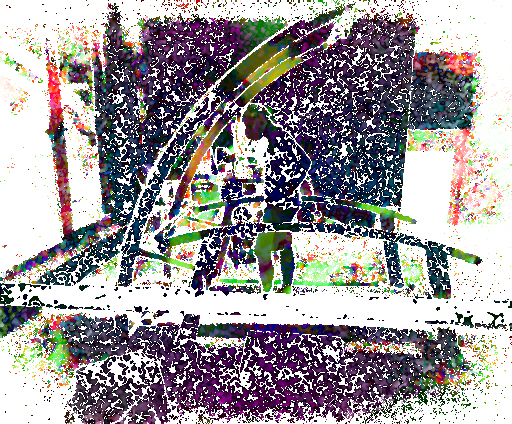
\includegraphics[width=\columnwidth, frame]{stage2-lab-sf-sv-pdflow-corrected.jpg}
		\caption{Stranska slika.}
	\end{subfigure}
	~
	\begin{subfigure}[t]{0.45\columnwidth}
		\centering
		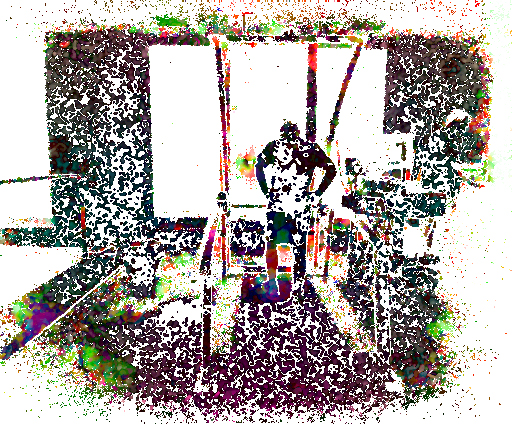
\includegraphics[width=\columnwidth, frame]{stage2-lab-sf-bv-pdflow-corrected.jpg}
		\caption{Hrbtna slika.}
	\end{subfigure}
	%~
	%\begin{subfigure}[t]{0.45\columnwidth}
	%	\centering
	%	\begin{tikzpicture}%[tdplot_main_coords, scale=0.5]
[x={(0.8cm,0.4cm)}, y={(0cm,1cm)}, z={(0.8cm,-0.4cm)}, scale=0.5]

\pgfmathtruncatemacro{\Divisions}{50};
\pgfmathsetmacro{\Cube}{5};
%\definecolor{mypurple}{RGB}{255,0,255};

	% Coordinate system
    \coordinate (O) at (0,0,0);
    \coordinate (oo) at (0,0,5);
    \coordinate (y) at (0,5,0);
    \coordinate (z) at (0,0,15);
    \coordinate (x) at (10,0,0);
    \draw [axis, thick] (O) -- (y) node [right] {$y$};
    \draw [axis] (O) -- (z) node [below] {$z$};
    \draw [axis] (O) -- (x) node [below] {$x$};
    \node (izhodisce) [below] at (O) {$\vec{O}$};
   
    
    \begin{scope}[canvas is yz plane at x=-\Cube/2]
    \shade[lower right=purple, lower left=blue, upper right=white, upper left=cyan] (-1,-1) rectangle (1,1);
    \clip (-\Cube/2,-\Cube/2) rectangle (\Cube/2,\Cube/2);
    \colorlet{BL}[RGB]{blue}
    \colorlet{BR}[RGB]{purple}
    \colorlet{TL}[RGB]{cyan}
    \colorlet{TR}[RGB]{white}
    \foreach \x in {1,...,\Divisions}
    {   \pgfmathtruncatemacro{\px}{(\x-1)/(\Divisions-1)*100}
    	\colorlet{B}[RGB]{BR!\px!BL}
    	\colorlet{T}[RGB]{TR!\px!TL}
    	\foreach \y in {1,...,\Divisions}
    	{   \pgfmathtruncatemacro{\py}{(\y-1)/(\Divisions-1)*100}
    		\fill[T!\py!B] ({-\Cube/2+\Cube*(\x-1)/\Divisions},{-\Cube/2+\Cube*(\y-1)/\Divisions}) rectangle ({-\Cube/2+\Cube*(\x+0.1)/\Divisions},{-\Cube/2+\Cube*(\y+0.1)/\Divisions});
    	}
    }
    \draw[thick] (-\Cube/2,-\Cube/2) rectangle (\Cube/2,\Cube/2);
    \end{scope}
    
    \begin{scope}[canvas is xz plane at y=\Cube/2]
    \clip (-\Cube/2,-\Cube/2) rectangle (\Cube/2,\Cube/2);
    \colorlet{BL}[RGB]{purple}
    \colorlet{BR}[RGB]{red}
    \colorlet{TL}[RGB]{white}
    \colorlet{TR}[RGB]{yellow}
    \foreach \x in {1,...,\Divisions}
    {   \pgfmathtruncatemacro{\px}{(\x-1)/(\Divisions-1)*100}
    	\colorlet{B}[RGB]{BR!\px!BL}
    	\colorlet{T}[RGB]{TR!\px!TL}
    	\foreach \y in {1,...,\Divisions}
    	{   \pgfmathtruncatemacro{\py}{(\y-1)/(\Divisions-1)*100}
    		\fill[T!\py!B] ({-\Cube/2+\Cube*(\x-1)/\Divisions},{-\Cube/2+\Cube*(\y-1)/\Divisions}) rectangle ({-\Cube/2+\Cube*(\x+0.1)/\Divisions},{-\Cube/2+\Cube*(\y+0.1)/\Divisions});
    	}
    }
    \draw[thick] (-\Cube/2,-\Cube/2) rectangle (\Cube/2,\Cube/2);
    \end{scope}
    
    \begin{scope}[canvas is xy plane at z=\Cube/2]
    \clip (-\Cube/2,-\Cube/2) rectangle (\Cube/2,\Cube/2);
    \colorlet{BL}[RGB]{cyan}
    \colorlet{BR}[RGB]{green}
    \colorlet{TL}[RGB]{white}
    \colorlet{TR}[RGB]{yellow}
    \foreach \x in {1,...,\Divisions}
    {   \pgfmathtruncatemacro{\px}{(\x-1)/(\Divisions-1)*100}
    	\colorlet{B}[RGB]{BR!\px!BL}
    	\colorlet{T}[RGB]{TR!\px!TL}
    	\foreach \y in {1,...,\Divisions}
    	{   \pgfmathtruncatemacro{\py}{(\y-1)/(\Divisions-1)*100}
    		\fill[T!\py!B] ({-\Cube/2+\Cube*(\x-1)/\Divisions},{-\Cube/2+\Cube*(\y-1)/\Divisions}) rectangle ({-\Cube/2+\Cube*(\x+0.1)/\Divisions},{-\Cube/2+\Cube*(\y+0.1)/\Divisions});
    	}
    }
    \draw[thick] (-\Cube/2,-\Cube/2) rectangle (\Cube/2,\Cube/2);
    \end{scope}
	    
\end{tikzpicture}
	%	\caption{Hrbtna slika.}
	%\end{subfigure}
	\caption[Stranska in hrbtna slika prostorskega toka lab. eksperimentov]{Stranska in hrbtna slika prostorskega toka laboratorijskih eksperimentov. Slike smo pridobili s programom \texttt{Scene-Flow-Impair} avtorja~\cite{jaimez2015primal}, ki smo ga prilagodili za Kinect V2 kamero. Sliki sta 8-bit RGB sliki. Amplitude hitrosti v posameznih oseh so normirane in normalizirane na intervalu $[0,255]$. Kanal B predstavlja komponento $\mu_x$, kanal G $\mu_y$, ter kanal R $\mu_z$ prostorskega toka $\vec{\mu}$. Beli slikovni elementi so neveljavni (ne vsebujejo podatka o globini).}
	\label{fig:stage2-lab-sf-pd}
\end{figure}

\begin{figure}[!htb]
	\centering
	\begin{subfigure}[t]{0.45\columnwidth}
		\centering
		
\includegraphics[width=0.5\columnwidth, frame]{./Slike/stage2-lab-sf-sv-flo-corrected.png}
		\caption{stranska slika}
		\label{fig:stage2-lab-sf-sv-flo}
	\end{subfigure}
	~
	\begin{subfigure}[t]{0.45\columnwidth}
		\centering
		
\includegraphics[width=0.5\columnwidth, frame]{./Slike/stage2-lab-sf-bv-flo-corrected.png}
		\caption{hrbtna slika}
		\label{fig:stage2-lab-sf-bv-flo}
	\end{subfigure}
	~
	\begin{subfigure}[t]{0.45\columnwidth}
		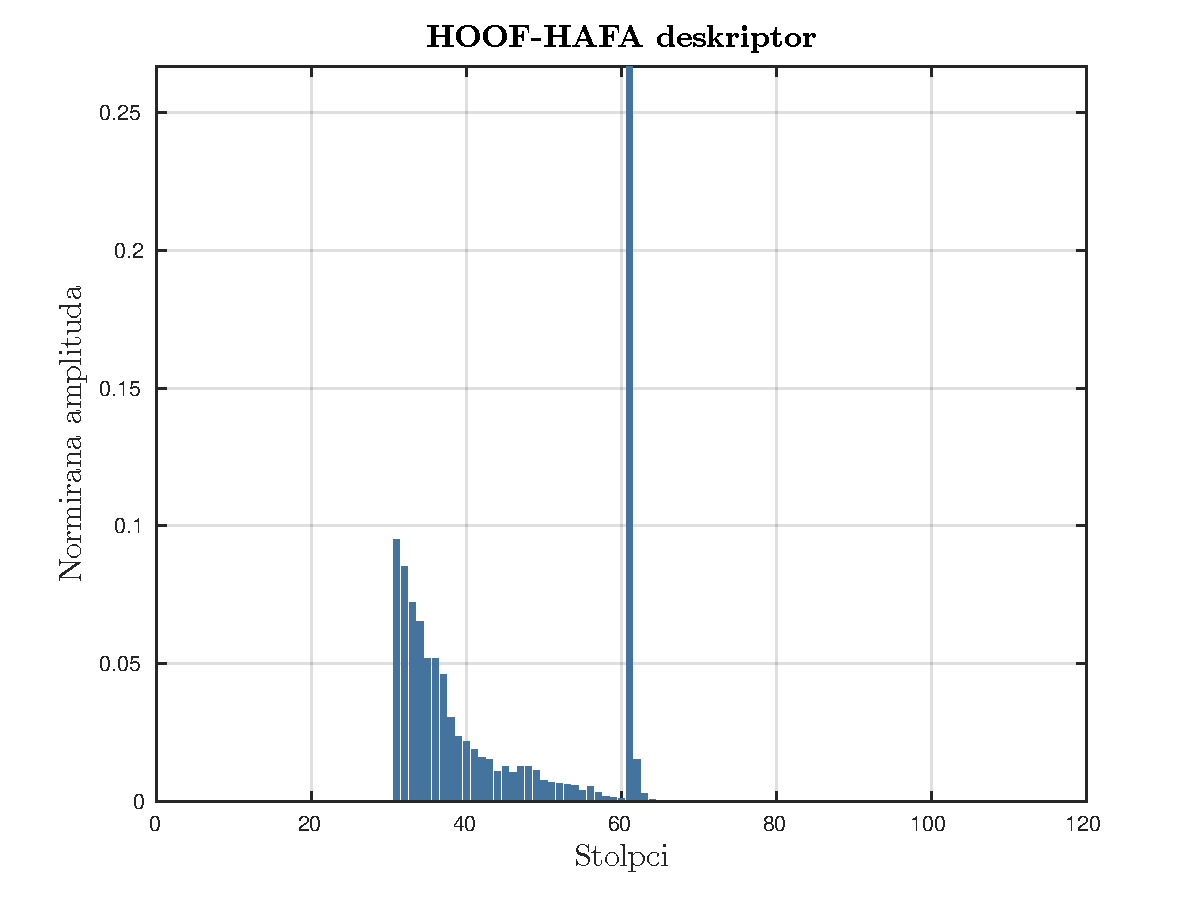
\includegraphics[width=\columnwidth]{stage2-lab-sv-sf-hist-sl}
		\caption{Histogram stranske slike.}
	\end{subfigure}
	~
	\begin{subfigure}[t]{0.45\columnwidth}
		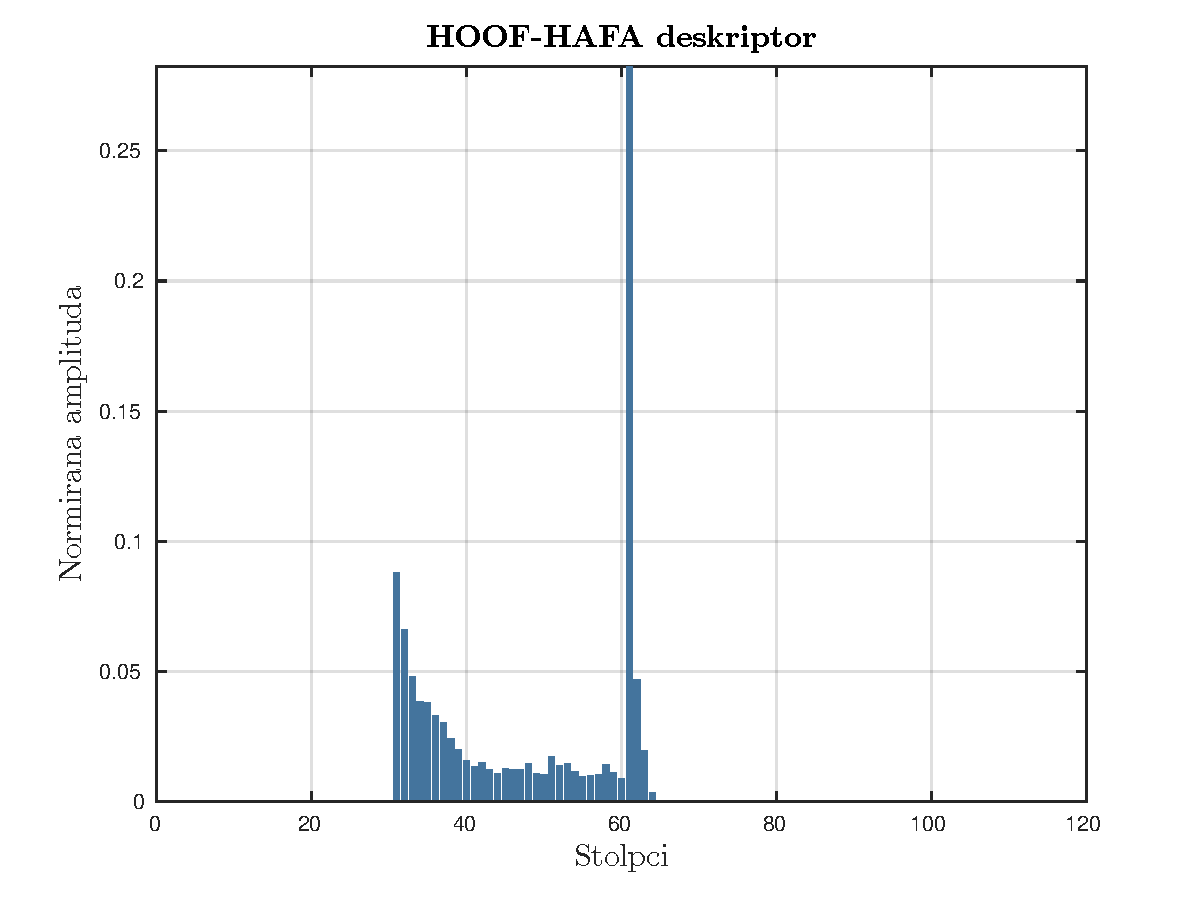
\includegraphics[width=\columnwidth]{stage2-lab-bv-sf-hist-sl}
		\caption{Histogram hrbtne slike.}
	\end{subfigure}
	\caption[Projekcije prostorskih tokov na slikovno ravnino]{Projekcija stranskega in hrbtnega prostorskega toka na slikovno ravnino. Gre za prostorska toka 24. stranske in hrbtne slike merjenca SUBJ1, ki sta že obrezani. V spodnjem levem kotu posamezne slike sta legendi barvnega kodiranja. Na sliki uporabljamo standardno barvno kodiranje, povzeto po~\cite{baker2011database}. Maksimalna amplituda prostorskega toka je na sliki  \subref{fig:stage2-lab-sf-sv-flo}) znašala \SI{10.4}{\m\per\s} in na \subref{fig:stage2-lab-sf-bv-flo}) \SI{9.4}{\m\per\s}. Projekcijama prostorskega toka pripadata izračunana HOOF-HAFA histograma.}
	\label{fig:prostorski-tok-stage2}
\end{figure}

\begin{figure}[!htb]
	\centering
	\resizebox{\columnwidth}{!}{\begin{tikzpicture}
% LAYERS
\pgfdeclarelayer{bg}
\pgfsetlayers{bg,main}
\tikzset{
	between/.style args={#1 and #2}{
		at = ($(#1)!0.5!(#2)$)
	}
}

% NODES
\node (slika) [input] at (0,0) {Slika\\$I(x,y)$};
\node (tracker) [block, right= of slika] {DS-KCF\\sledilnik};
%\node (tarca) [block, right= of tracker] {Področje\\ tarče $x^{p}$};

\node (of) [block, right= of tracker] {Prostorski\\ tok};
\node (hoof) [block, right= of of] {HOOF-HAFA\\deskriptorji};


\node (ucenje) [block, right=of hoof] {\nurbf};
\node (kalman) [block, right= of ucenje] {Gaussov\\ filter};


\node (rezultat) [output, right= of kalman] {Rezultat};

% arrows
\draw [arrow] (slika) -- (tracker);
\draw [arrow] (tracker) -- (of);
%\draw [arrow] (tarca) -- (of);
\draw [arrow] (of) -- (hoof);
\draw [arrow] (hoof) -- (ucenje);
\draw [arrow] (ucenje) -- (kalman);
\draw [arrow] (kalman) -- (rezultat);
\end{tikzpicture}}
	\caption[Diagram testiranja s prostorskim tokom za eksperimente 2. faze]{Diagram testiranja procesiranja s prostorskim tokom za eksperimente 2. faze.}
	\label{fig:diagram-procesiranja-sf-stage2}
\end{figure}
 
Modele obeh postopkov smo učili s postopkom \nurbf, kjer smo za Gaussov filter uporabili $\sigma=5$ in za največje število podpornih vektorjev $\numax =0.5$ (\SI{50}{\%} podpornih vektorjev). Podobno kot v eksperimentih 1. faze smo tudi tu naučili \num{6} elementarnih modelov, in sicer: \textit{eem} modele, ki predvidevajo porabo energije v \si{\kcal\per\min}, \textit{sv} modele za stransko kamero in \textit{bv} modele za hrbtno kamero. %ter \textit{lag} modele z upoštevanjem časovne zakasnitve.

Vse tipe eksperimentov smo križno testirali glede na enak tip eksperimenta, le z drugim zornim kotom kamere. Uporabljen zorni kot kamere za križno testiranje je v imenih modelov zapisan v oklepajih.  Rezultate smo filtrirali z Gaussovim jedrom $\sigma=5$. 

Modele smo testirali po treh različnih protokolih. S prvim protokolom smo preverjali neodvisnost od časovnega povečevanja porabe, z drugim pa ravno obratno. S tretjim protokolom smo želeli pokazati delovanje posplošenega modela na različnih merjencih.


\paragraph{Protokol 1.}
Za testne vzorce vzamemo vsak 3. vzorec fiziološkega parametra in slike iz posameznega posnetka. Ostale vzorce uporabimo pri učenju. Rezultate vseh 6 meritev povprečimo.

\paragraph{Protokol 2.}
Za učne vzorce izberemo prvih \SI{70}{\%} vzorce in za testne naslednjih \SI{30}{\%}. Rezultate vseh 6 meritev povprečimo.

\paragraph{Protokol 3.}
Uporabimo protokol 1, pri čemer učimo na prvih štirih meritvah in testiramo na zadnjih dveh. Rezultatov ne povprečimo.

\begin{comment}
\subsubsection{Določitev zakasnitve fiziološkega odziva}
Določitve zakasnitve fiziološkega odziva smo se, glede na eksperimente 1. faze, tu lotili nekoliko drugače. Na podlagi protokola izvajanja meritev, smo pridobili podatke eno minutnega mirovanja posameznega merjenca z vzorčno frekvenco \SI{0.2}{\hertz}. Kljub temu, da je signal v stacionarnem stanju, je nihajoč zaradi narave fiziologije. Signal mirovanja smo interpolirali na vzorčno frekvenco \SI{1}{\hertz}. Določili smo mu srednjo vrednost in vrednost treh standardnih odklonov. S tem smo dobili interval nedoločenosti, v katerem ne moremo določiti ali je pri spremembi amplitude signala prišlo zaradi fizioloških dejavnikov ali zaradi dejanskega odziva na vzbujalni signal. 

Na podlagi slik~\ref{fig:lag-estimation-stage2}, smo zakasnitev za posamezno meritev določili kot časovni interval od trenutka spremembe hitrosti tekalne steze do trenutka, ko je bila vrednost fiziološkega parametra prvič nad intervalom nedoločenosti. Zakasnitev smo, zaradi treh standardnih odklonov, lahko določili s \SI{99.73}{\%} zagotovostjo za posameznega merjenca. Zakasnitve vseh merjencev smo povprečili in dobili vrednost \SI{26}{\s} za energijsko porabo.

\begin{figure}[!htbp]
	\centering
	\begin{subfigure}[t]{0.45\columnwidth}
		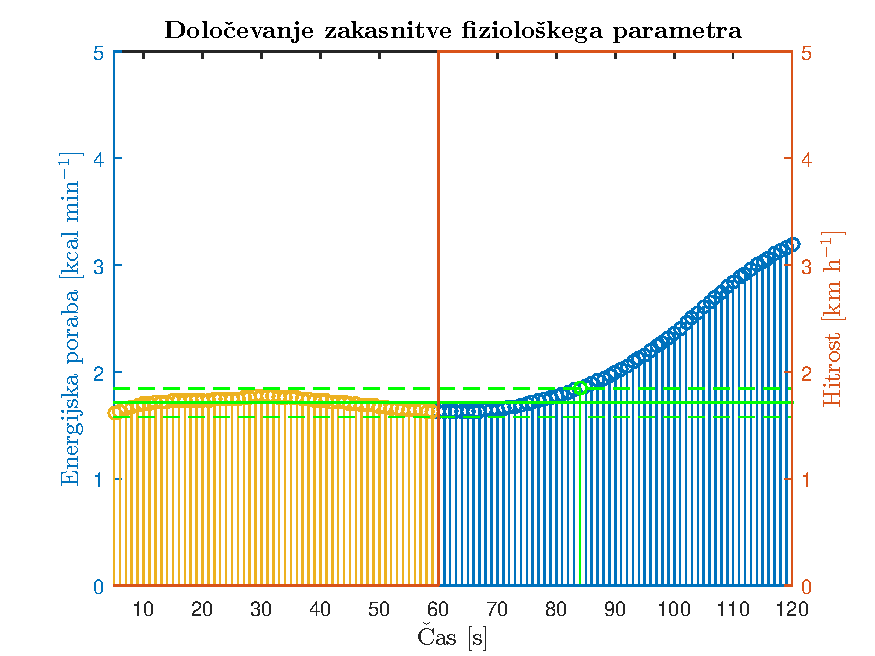
\includegraphics[width=\columnwidth]{stage2-lag-estimation-1-eem-sl}
		\caption{Zakasnitev za subjekt 1.}
		\label{fig:lag-estimation-1-eem}
	\end{subfigure}
	~
	\begin{subfigure}[t]{0.45\columnwidth}
		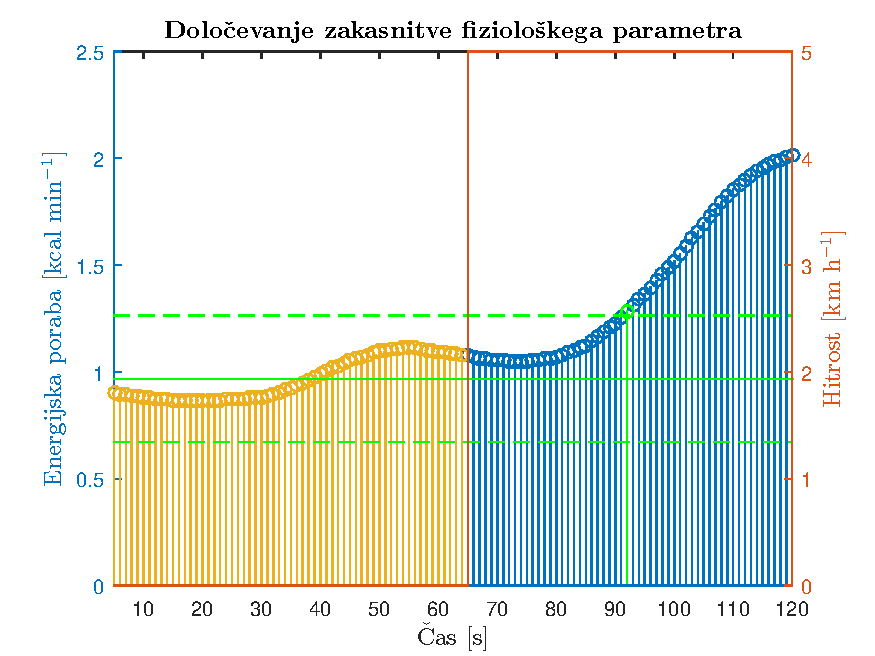
\includegraphics[width=\columnwidth]{stage2-lag-estimation-2-eem-sl}
		\caption{Zakasnitev za subjekt 2.}
		\label{fig:lag-estimation-2-eem}
	\end{subfigure}
	~
	\begin{subfigure}[t]{0.45\columnwidth}
		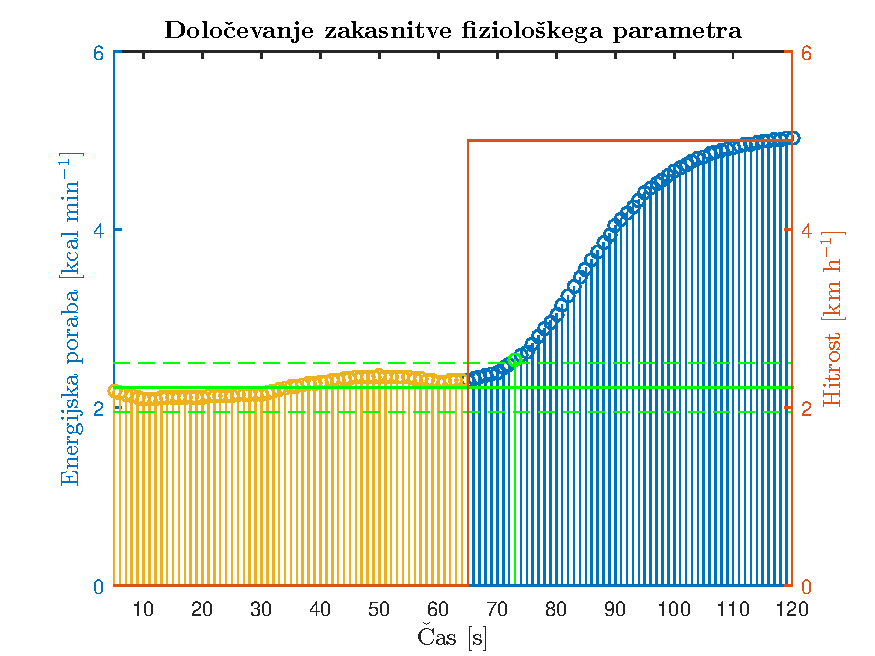
\includegraphics[width=\columnwidth]{stage2-lag-estimation-3-eem-sl}
		\caption{Zakasnitev za subjekt 3.}
		\label{fig:lag-estimation-3-eem}
	\end{subfigure}
	~
	\begin{subfigure}[t]{0.45\columnwidth}
		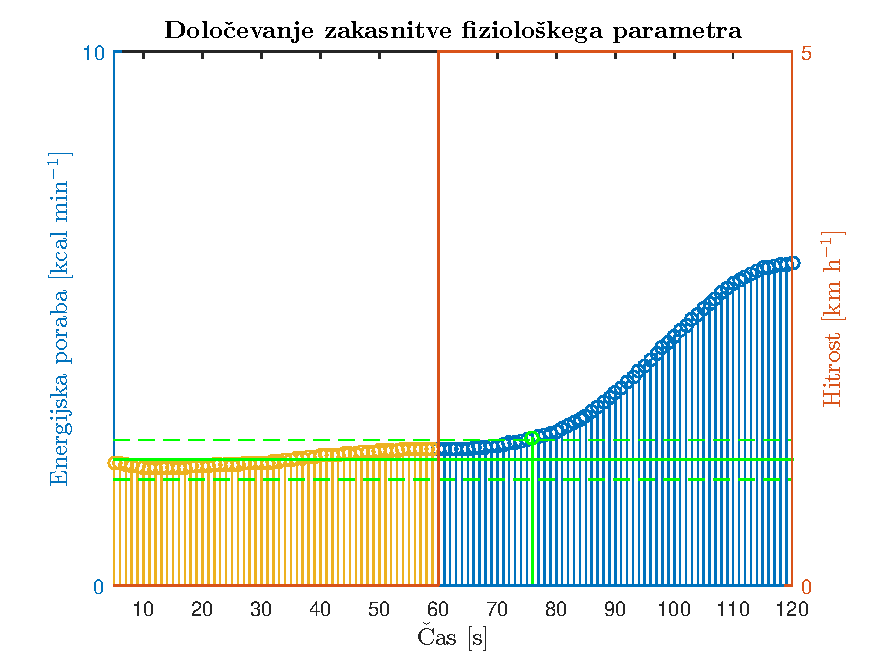
\includegraphics[width=\columnwidth]{stage2-lag-estimation-4-eem-sl}
		\caption{Zakasnitev za subjekt 4.}
		\label{fig:lag-estimation-4-eem}
	\end{subfigure}
	~
	\begin{subfigure}[t]{0.45\columnwidth}
		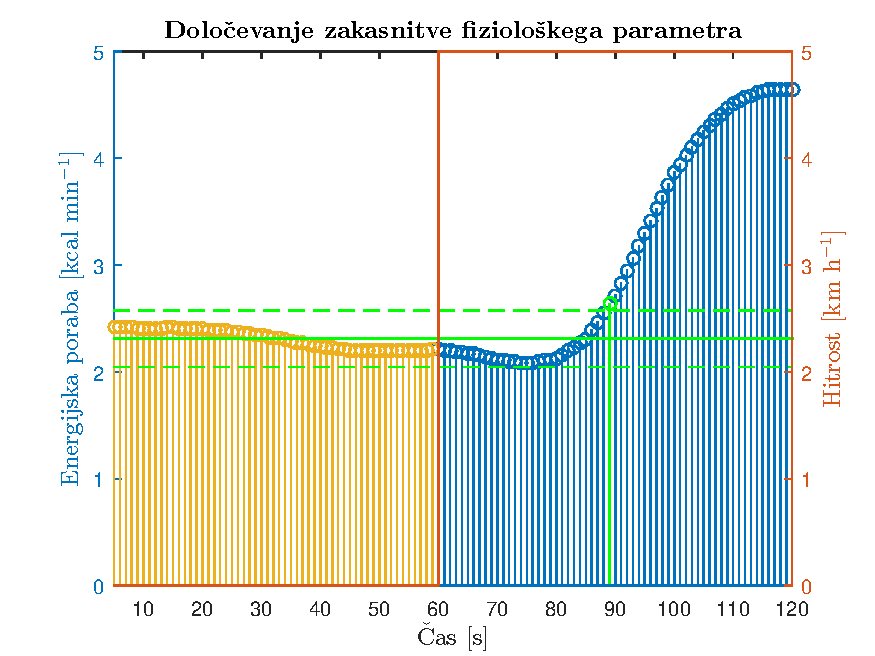
\includegraphics[width=\columnwidth]{stage2-lag-estimation-5-eem-sl}
		\caption{Zakasnitev za subjekt 5.}
		\label{fig:lag-estimation-5-eem}
	\end{subfigure}
	~
	\begin{subfigure}[t]{0.45\columnwidth}
		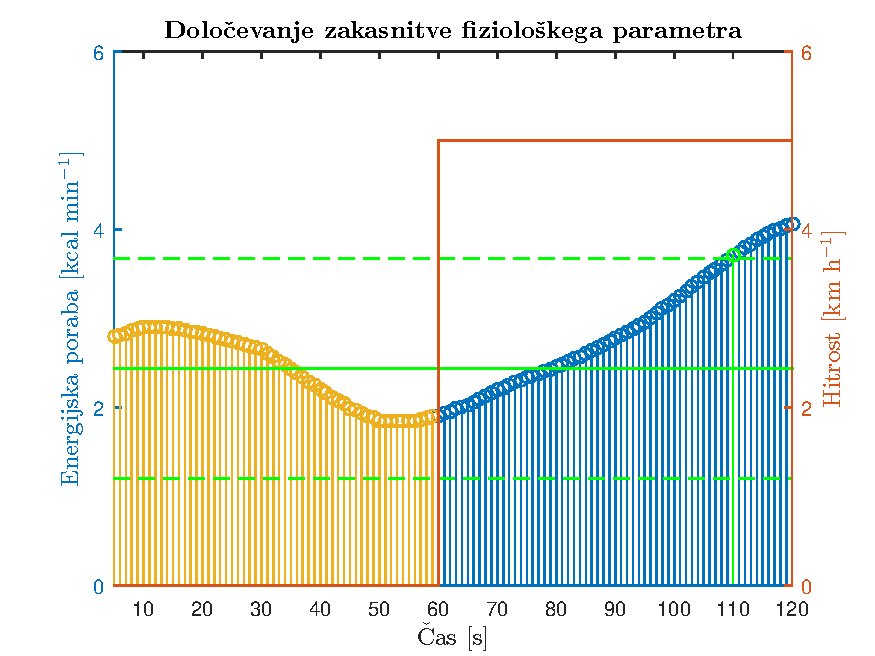
\includegraphics[width=\columnwidth]{stage2-lag-estimation-6-eem-sl}
		\caption{Zakasnitev za subjekt 6.}
		\label{fig:lag-estimation-6-eem}
	\end{subfigure}
	\caption[Prikaz določitve zakasnitve za posameznega merjenca]{Prikaz določitve zakasnitve za posameznega merjenca. Zakasnitev za posamezno meritev smo določili kot časovni interval od trenutka spremembe hitrosti tekalne steze do trenutka, ko je bila vrednost fiziološkega parametra prvič nad intervalom nedoločenosti. Interval nedoločenosti je prikazan z zelenimi horizontalnimi linijami. Rumeni vzorci so vzorci enominutnega mirovanja. Sledijo modri vzorci pri hoji na tekalni stezi s hitrostjo \SI{5}{\km\per\hour}. Spremenba hitrosti tekalne steze je prikazana z rdečim signalom.}
	\label{fig:lag-estimation-stage2}
\end{figure}
\end{comment}









\subsection{Terenski eksperimenti}
Pri terenskih eksperimentih smo postopek z optičnim tokom in postopek s prostorskim tokom preverili še v realističnem okolju. Šest igralcev je igralo squash igro z dvema setoma. Tako smo pridobili podatke za 3 igre, ki so trajale \SI{16}{\min} \SI{14}{\min} in \SI{11}{\min}. 

Postopki procesiranja in protokoli procesiranja so enaki kot v laboratorijskih eksperimentih 2. faze. Delovanje sledilnikov lahko vidimo na sliki~\ref{fig:stage2-field-tracked}. Pripadajoči optični in prostorski tok sta prikazana na sliki~\ref{fig:stage2-field-sfof}. Na sliki~\ref{fig:stage2-field-hist} sta prikazana pripadajoča histograma.

\begin{figure}[!htb]
	\centering
	\begin{subfigure}{0.45\columnwidth}
		\centering
		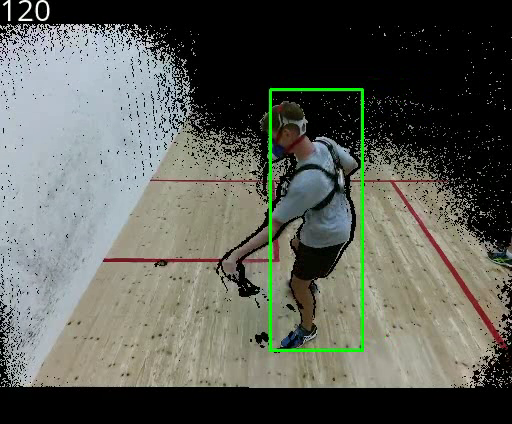
\includegraphics[width=\columnwidth]{stage2-field-of-left-tracked.png}
		\caption{KCF sledilnik}
	\end{subfigure}
	~
	\begin{subfigure}{0.45\columnwidth}
		\centering
		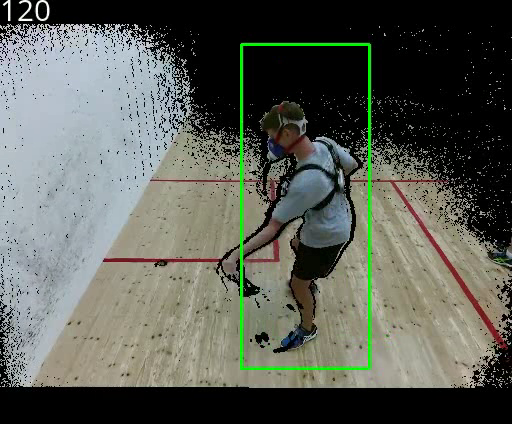
\includegraphics[width=\columnwidth]{stage2-field-sf-left-tracked.png}
		\caption{DS-KCF sledilnik.}
	\end{subfigure}
	\caption[Predstavitev delovanja KCF in DS-KCF sledilnikov]{Predstavitev delovanja KCF in DS-KCF sledilnikov za terenske eksperimente. Za primerjavo sledilnikov sta prikazani 120. sliki leve kamere prvega seta 2. igre za merjenca SUBJ9. Zelena okvirja prikazujeta detektirani področji za posamezen sledilnik. Opazimo, da sta področji različni.}
	\label{fig:stage2-field-tracked}
\end{figure}



\begin{figure}[!htb]
	\centering
	\begin{subfigure}[t]{0.3\columnwidth}
		\centering
		
\includegraphics[width=\columnwidth, frame]{./Slike/stage2-field-of-svbv-flo-corrected.png}
		\caption{Optični tok.}
		\label{fig:stage2-field-of}
	\end{subfigure}
	~
	\begin{subfigure}[t]{0.3\columnwidth}
		\centering
		
\includegraphics[width=\columnwidth, frame]{./Slike/stage2-field-sf-svbv-flo-corrected.png}
		\caption{Projekcija prostorskega toka.}
		\label{fig:stage2-field-pd}
	\end{subfigure}
	~
	\begin{subfigure}[t]{0.3\columnwidth}
		\centering
		
\includegraphics[width=\columnwidth, frame]{./Slike/stage2-field-sf-pd-tr-corrected.jpg}
		\caption{Prostorski tok.}
	\end{subfigure}
	\caption[Optični tok, prostorski tok in njegova projekcija]{Optični tok, prostorski tok in njegova projekcija na slikovno ravnino. V spodnjem levem kotu optičnega tok in projekcije prostorskega toka sta legendi barvnega kodiranja. Uporabljamo standardno barvno kodiranje, povzeto po~\cite{baker2011database}. Maksimalna amplituda optičnega toka na sliki  \subref{fig:stage2-field-of}) je  \SI{10}{ppf}. Maksimalna amplituda projekcije prostorskega toka je \SI{13.7}{\m\per\s}. Sliko prostorskega toka \subref{fig:stage2-field-pd}) smo pridobili s programom \texttt{Scene-Flow-Impair} avtorja~\cite{jaimez2015primal}, ki smo ga prilagodili za Kinect V2 kamero. Slika je 8-bitna RGB. Amplitude hitrosti v posameznih oseh so normirane in normalizirane na intervalu $[0,255]$. Kanal B predstavlja komponento $\mu_x$, kanal G $\mu_y$, ter kanal R $\mu_z$ prostorskega toka $\vec{\mu}$. Beli slikovni elementi so neveljavni (ne vsebujejo podatka o globini).}
	\label{fig:stage2-field-sfof}
\end{figure}



\begin{figure}[!htb]
	\centering
	\begin{subfigure}[t]{0.45\columnwidth}
		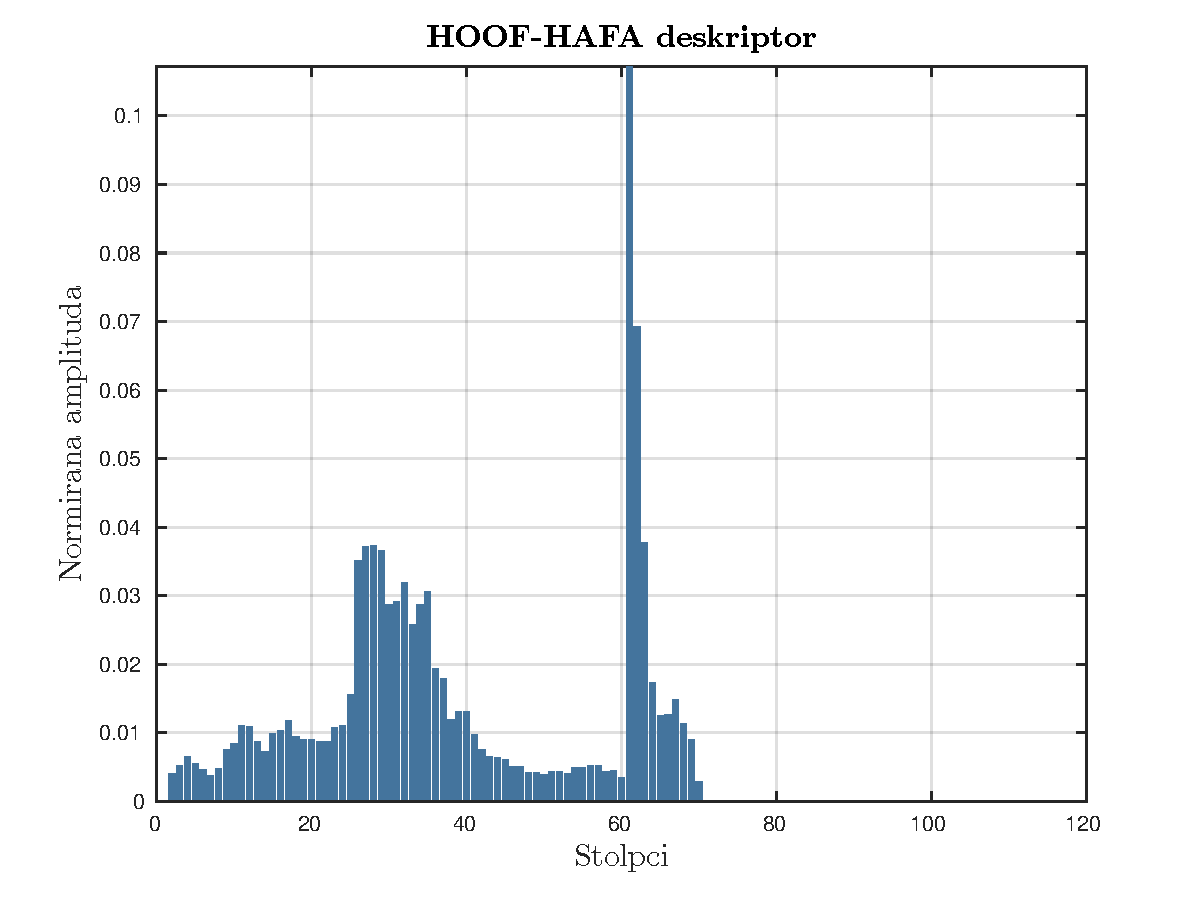
\includegraphics[width=\columnwidth]{stage2-field-bv-of-hist-sl}
		\caption{Histogram optičnega toka.}
	\end{subfigure}
	~
	\begin{subfigure}[t]{0.45\columnwidth}
		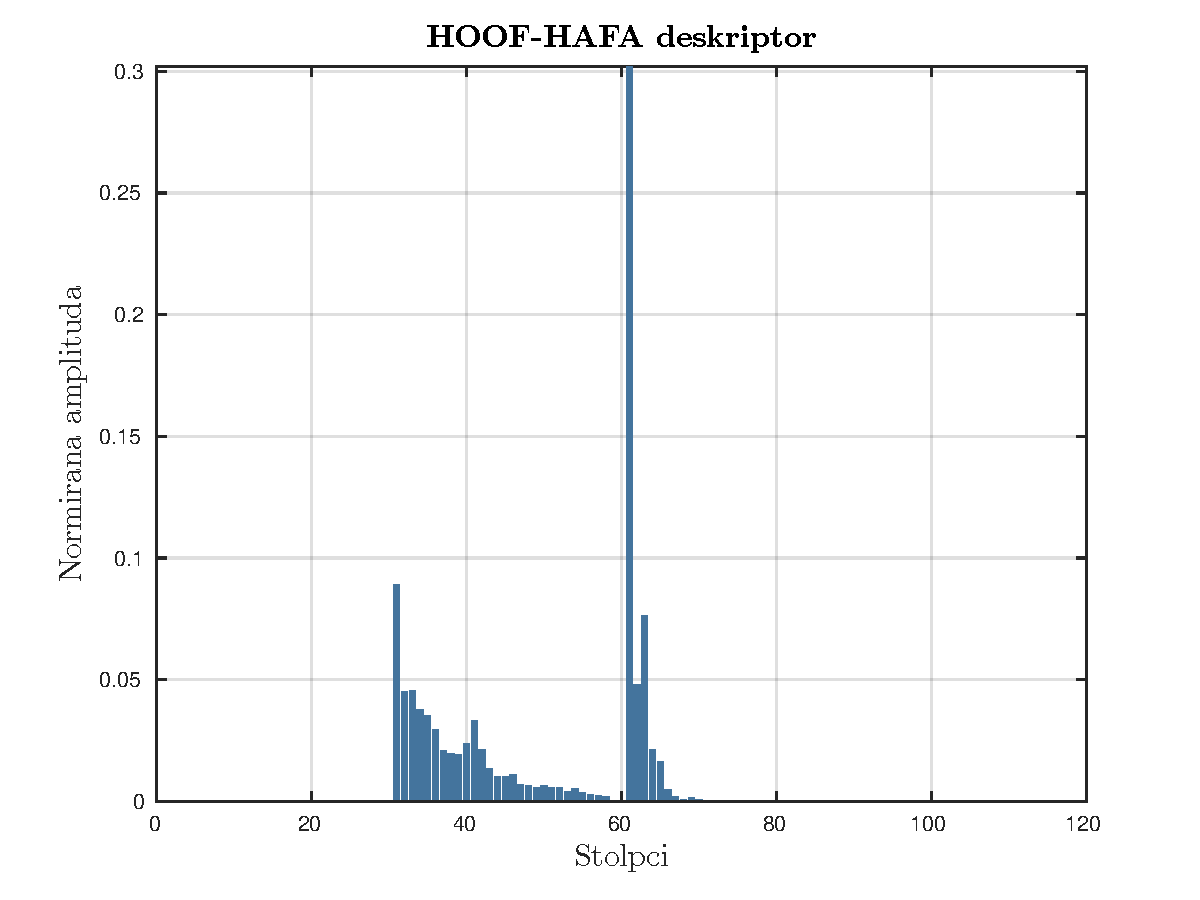
\includegraphics[width=\columnwidth]{stage2-field-bv-sf-hist-sl}
		\caption{Histogram prostorskega toka.}
	\end{subfigure}
	\caption[Histograma optičnega in projekcije prostorskega toka]{Histograma optičnega in projekcije prostorskega toka. Histogram za optični tok smo dobili iz slike~\ref{fig:stage2-field-sfof}\subref{fig:stage2-field-of}). Histogram projekcije prostorskega toka smo dobili iz slike~\ref{fig:stage2-field-sfof}\subref{fig:stage2-field-pd}}
	\label{fig:stage2-field-hist}
\end{figure}

\begin{comment}
\begin{figure}[!htb]
	\centering
	\begin{subfigure}[t]{0.45\columnwidth}
		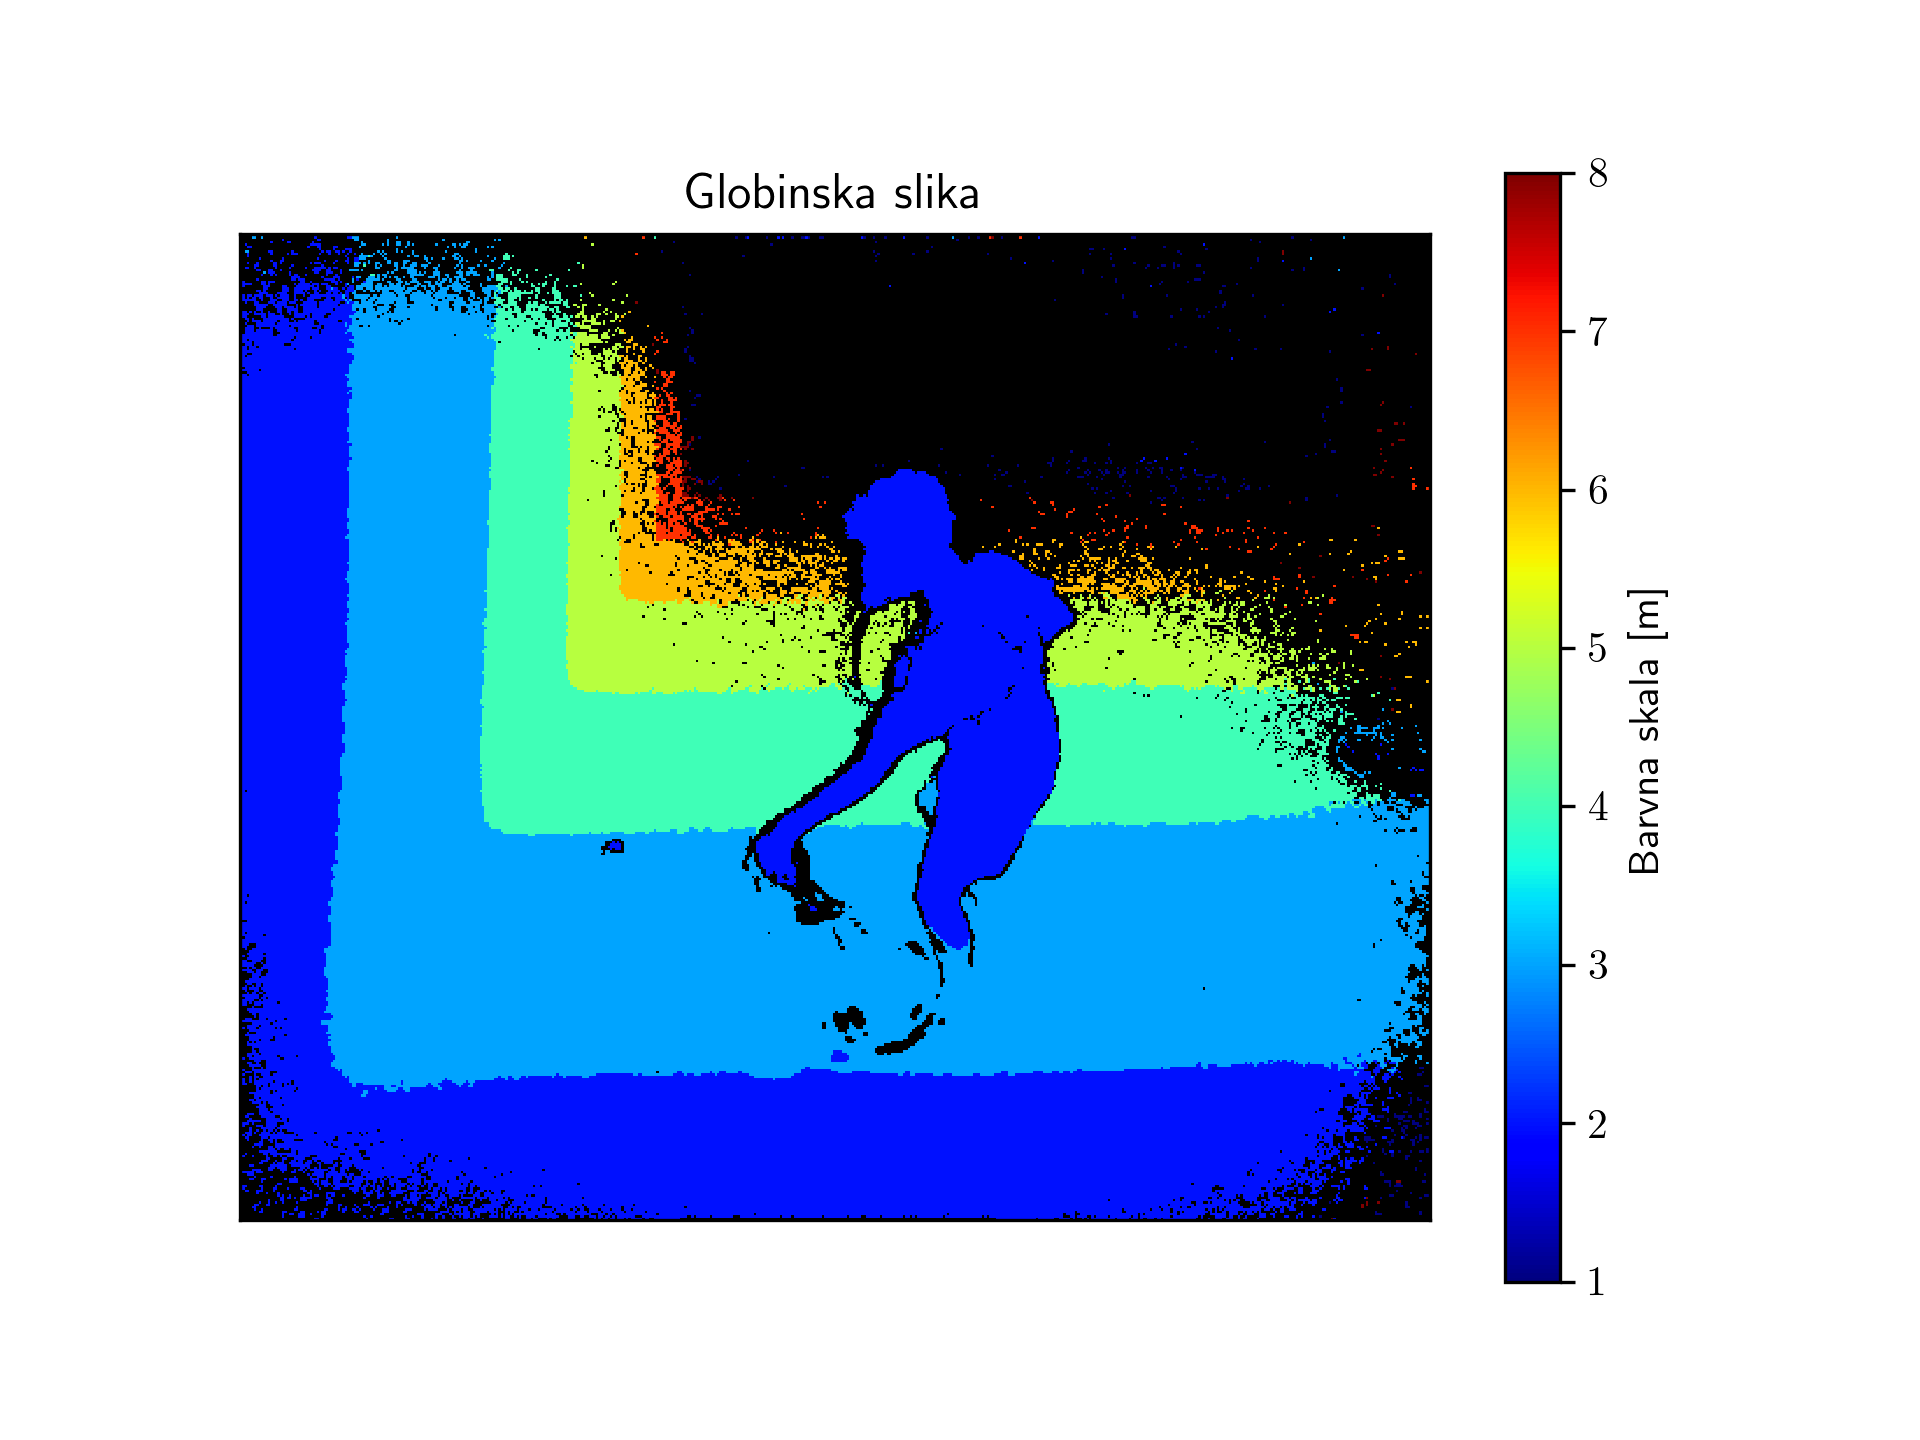
\includegraphics[width=1.2\columnwidth]{stage2-field-left-depth-sl}
		\caption{Stranska slika.}
	\end{subfigure}
	~
	\begin{subfigure}[t]{0.45\columnwidth}
		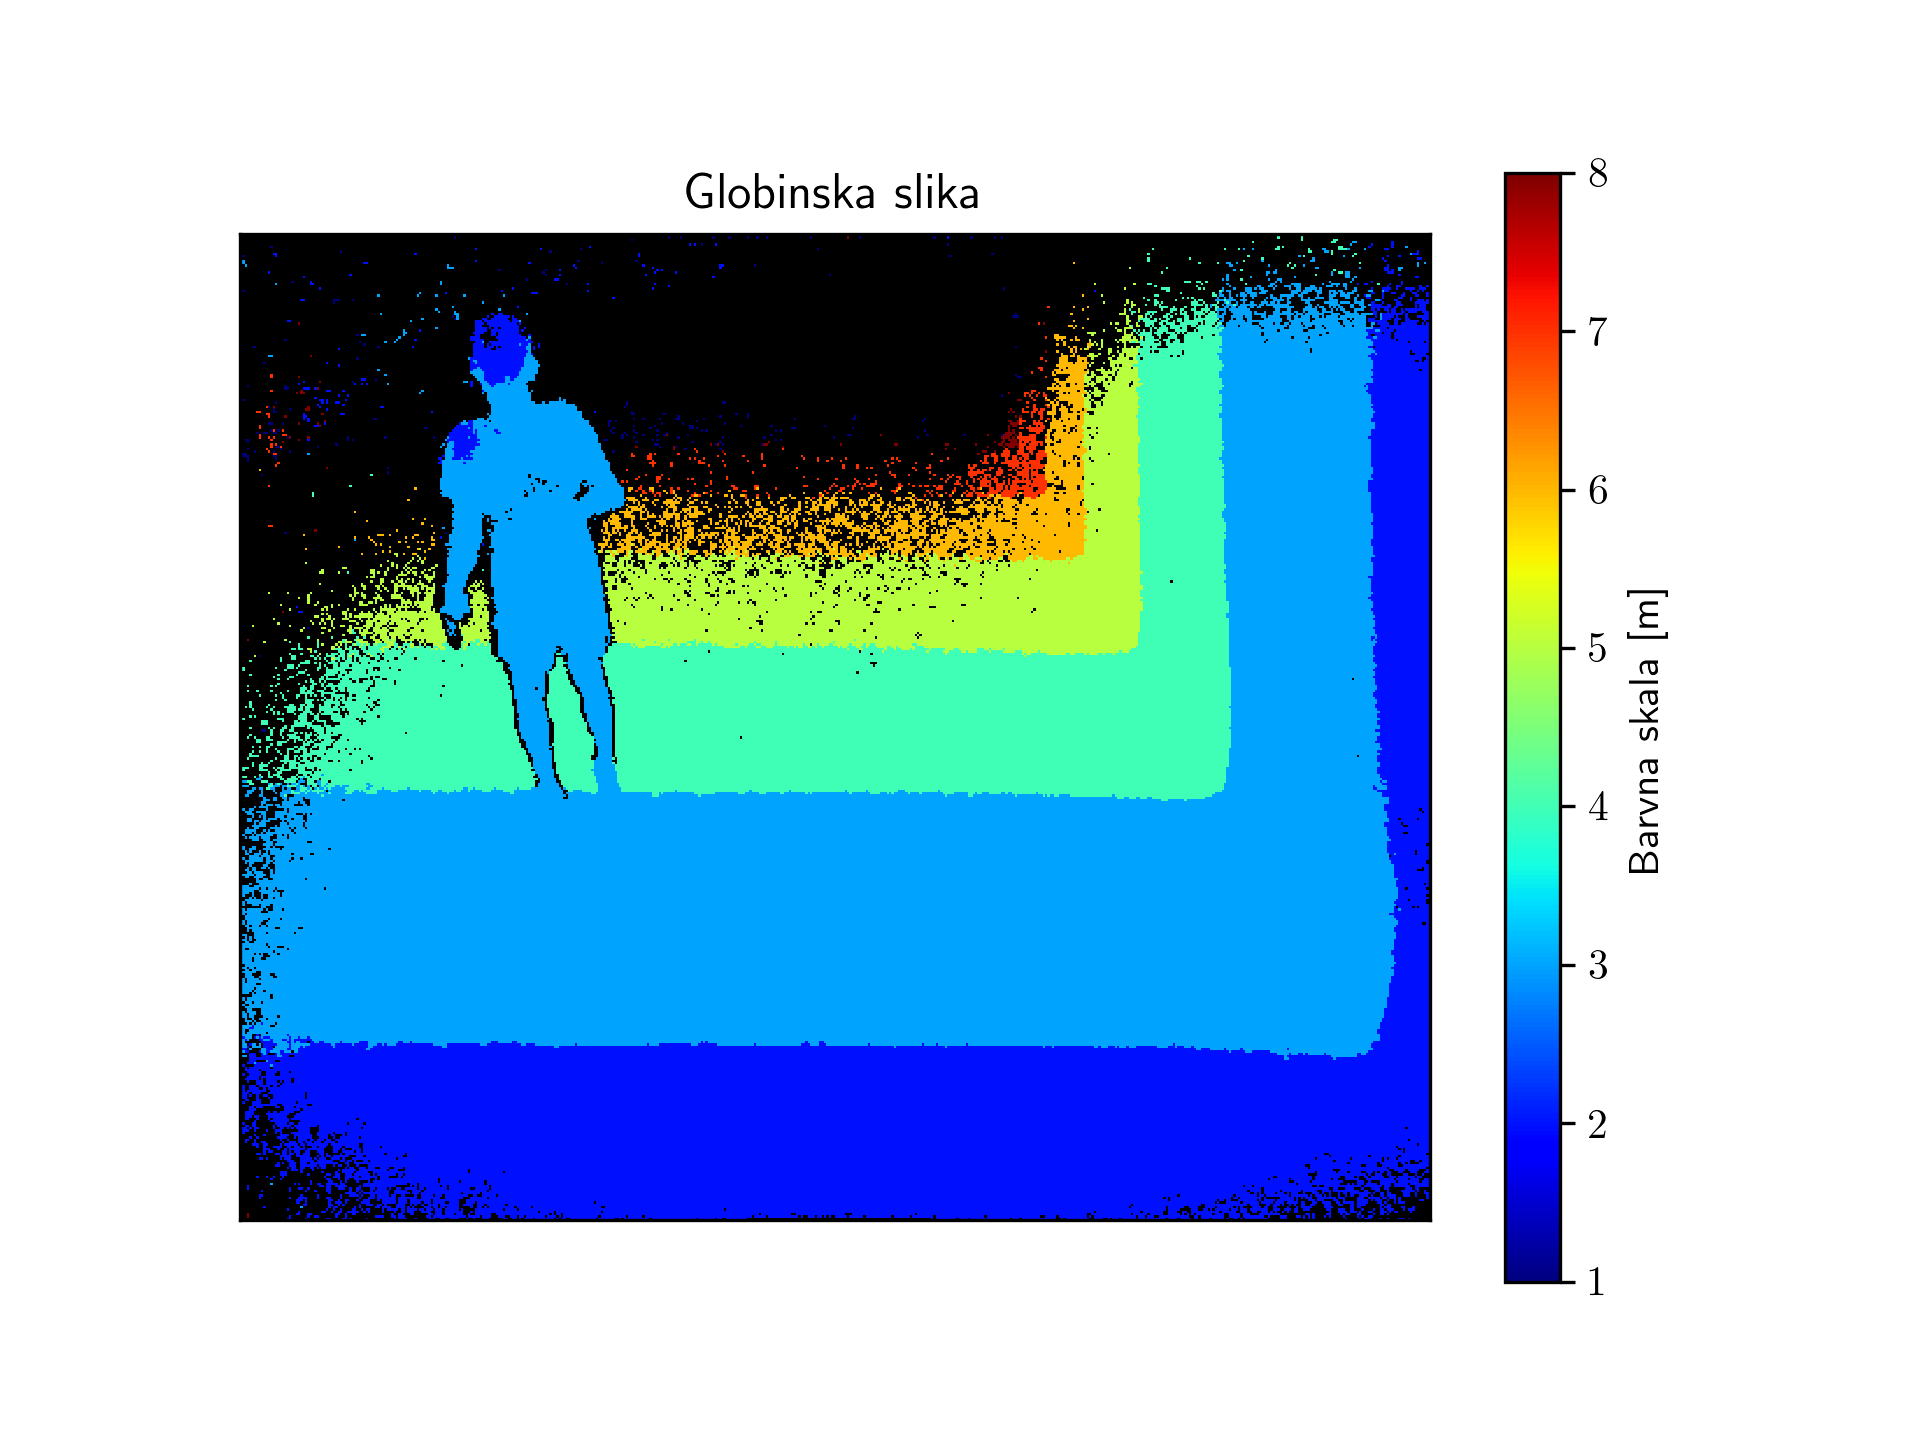
\includegraphics[width=1.2\columnwidth]{stage2-field-right-depth-sl}
		\caption{Hrbtna slika.}
	\end{subfigure}
	\caption[Stranska in hrbtna globinska slika pri terenskih testih 2. faze]{Stranska in hrbtna globinska slika pri terenskih testih 2. faze.}
	\label{fig:stage2-field-of-depth}
\end{figure}
\end{comment}



\subsubsection{Pridobivanje podatkov.}
\paragraph{Fiziolo\v{ski} parametri.}
Fiziološke parametre smo pridobili s pomočjo prenosnega sistema za direktno ergospirometrijo tipa ``breath  by breath'' Cosmed K4B2. Sistem je prikazan na sliki~\ref{fig:maske}. Frekvenca vzorčenja se je spreminjala, v povprečju pa je znašala \SI{0.5}{\hertz}. S testom smo pridobili podatke energijske porabe šestih različnih merjencev z oznakami: SUBJ1, SUBJ2, SUBJ7, SUBJ8, SUBJ9 in SUBJ10.


\begin{figure}[!htb]
	\centering
	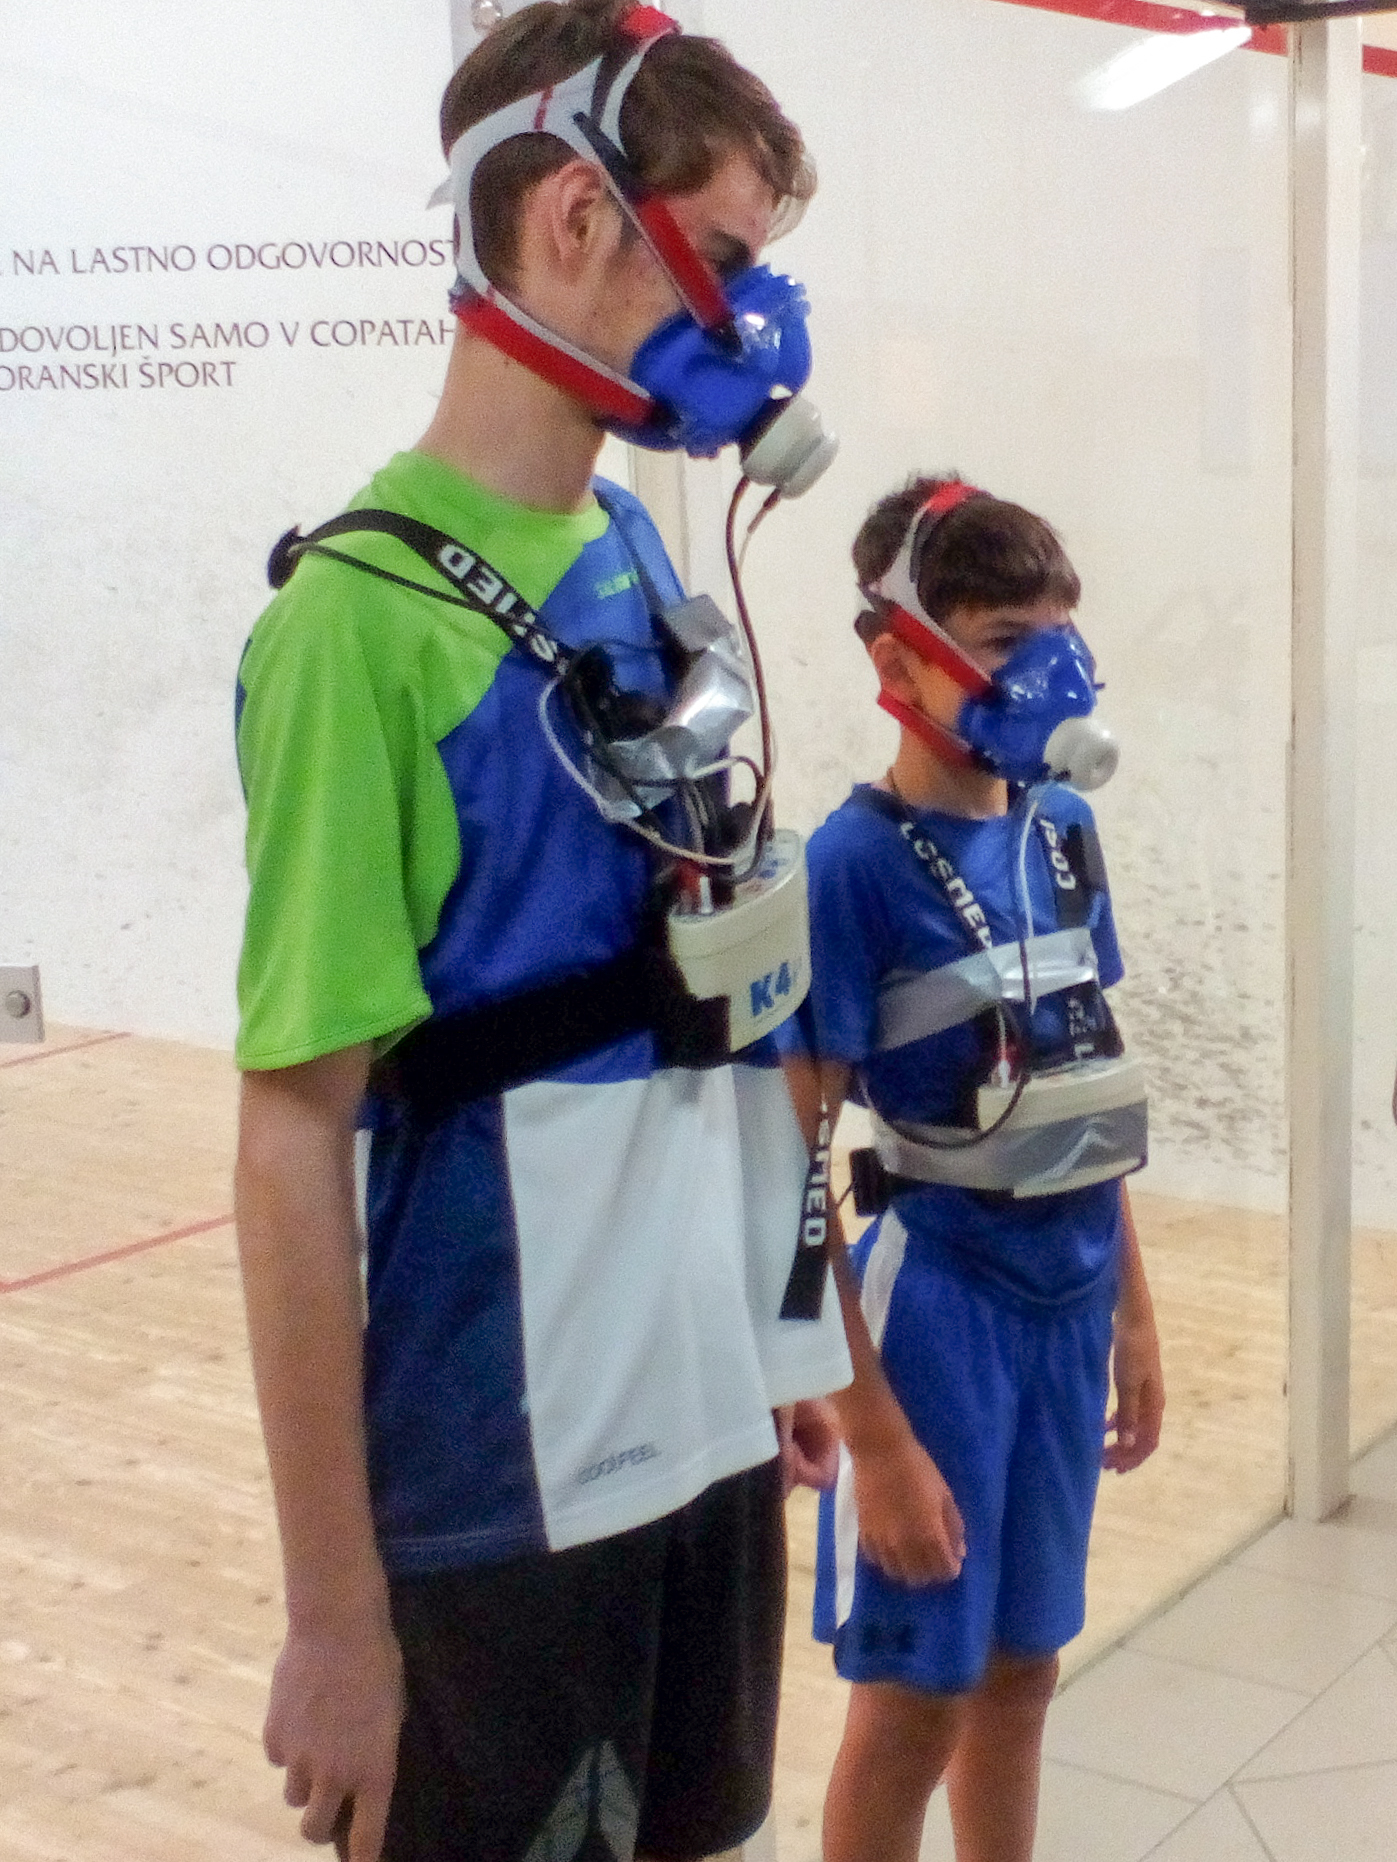
\includegraphics[width=0.4\columnwidth]{./Slike/squash-maske-corrected.jpg}	
	\caption[Prenosni sistem za direktno ergospirometrijo]{Prenosni sistem za direktno ergospirometrijo tipa ``breath  by breath'' Cosmed K4B2.}
	\label{fig:maske}
\end{figure}

\paragraph{Video posnetki.}
Igrišče smo snemali z dvema Microsoft Xbox Kinect V2 kamerama, ki sta bili oddaljeni ena od druge za približno \SI{2}{m}. Vsaka kamera je pokrivala svojo polovico igrišča. Razdalja od tal je znašala približno \SI{3}{m}. Kameri sta bili tako pozicionirani nad zaščitnim steklom. S tem nismo dobili odbojev laserskih žarkov, ki so namenjeni za pridobivanje globinske slike. Kot $\theta$ (rotacija okoli x osi) je bil približno $30\stopinj$ tako, da so kamere pokrivale prvo polovico igrišča do linije serviranja. Postavitev kamer je prikazana na sliki~\ref{fig:field-postavitev-kamer}.

\begin{figure}[!htb]
	\centering
	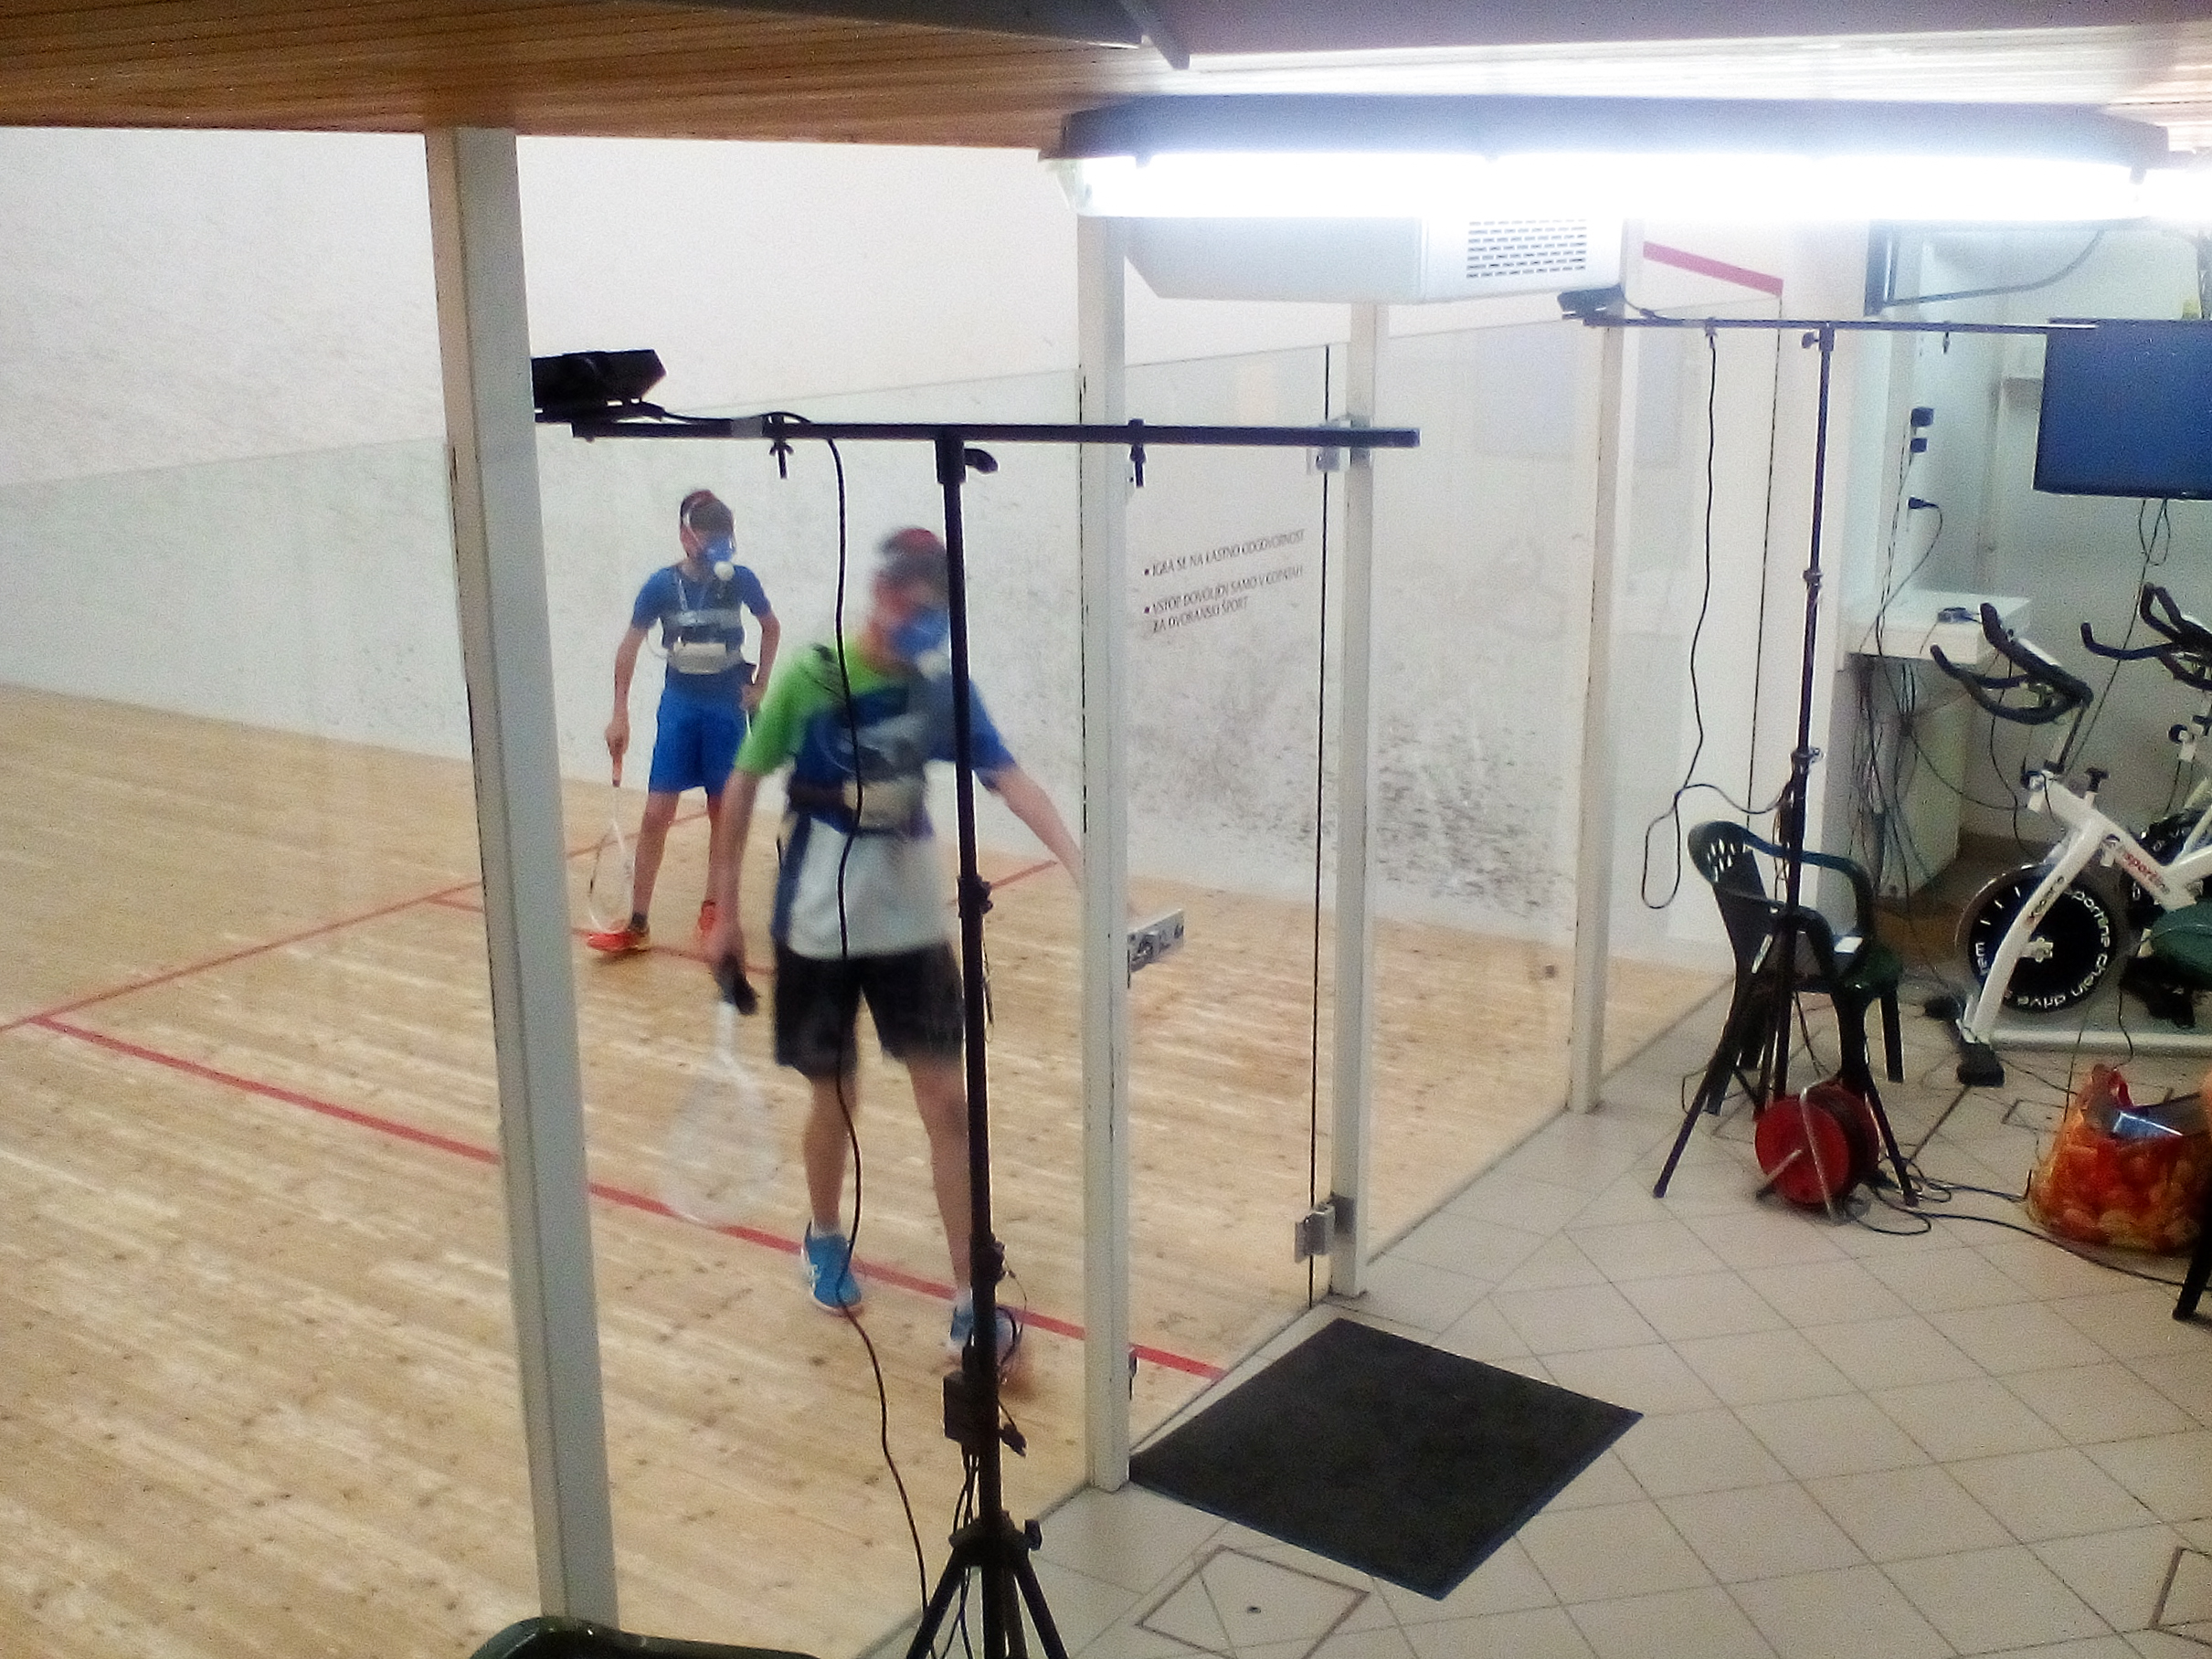
\includegraphics[width=0.6\columnwidth]{squash-postavitev-corrected.jpg}	
	\caption[Postavitev Kinect kamer pri terenskih testih 2. faze]{Postavitev Kinect kamer pri terenskih testih 2. faze.}
	\label{fig:field-postavitev-kamer}
\end{figure}


Pridobili smo barvne RGB in globinske DEPTH slike. Snemali smo v ločljivosti $512 \times 424$. Hitrost posnetkov je znašala \SI{30}{fps}. Kameri smo časovno sinhronizirali po NTP protokolu.



\paragraph{Protokol meritev.}
Posamezno igro smo pričeli s 5 minutnim ogrevalnim tekom. Sledilo je igranje na dva seta do 10 dobljenih točk z upoštevanjem dveh točk razlike. Med setoma so igralci počivali 2 minute. Ogrevanja in počivanja s kamerami nismo merili. Seta posamezne igre smo združili v en posnetek.

